%!TEX ROOT=formularioMatematica.tex

\section{Esercizi}
Questa sezione è dedicata ad alcuni esercizi con relativa risoluzione e spiegazione. Il suo scopo
è quello di chiarire i concetti teorici con esempi pratici.

\subsection*{\hyperref[sec:gen]{Generale}}\label{ex:generale}

\subsubsection*{\hyperref[subsec:gen:prodnot]{Prodotti notevoli}}
\paragraph{Esercizio 1}
Si scompongano il seguenti polinomi usando i prodotti notevoli.
\begin{equation}\label{eq:ex:prodnot1}
18x^3 - 4 -8x + 9x^2
\end{equation}
\begin{equation}\label{eq:ex:prodnot2}
a^2x^2 - a^2y^2 - b^2x^2 + b^2y^2
\end{equation}
% Reset the counter
\setcounter{equation}{0}
\divisor

Per semplificare \eqref{eq:ex:prodnot1} innanzitutto riscriviamo il polinomio in modo decrescente
\begin{equation*}
18x^3 + 9x^2- 8x - 4
\end{equation*}
Ora possiamo notare che i primi due elementi sono semplificabili, così come anche i secondi due per 
uno stesso fattore.
\begin{equation*}
\underbrace{18x^3 + 9x^2}_{9x^2(2x + 1)} \overbrace{- 8x - 4}^{-4(2x + 1)} = 
(9x^2 - 4)(2x + 1)
\end{equation*}
Ora abbiamo solo un altro prodotto da semplificare. Ricordando che $a^2-b^2 = (a-b)(a+b)$ possiamo
espandere la prima parentesi
\begin{equation*}
\boxed{(3x-2)(3x+2)(2x+1)}
\end{equation*}
Per semplificare \eqref{eq:ex:prodnot2} possiamo raccogliere i coefficienti di $x$ e $y$
\begin{equation*}
a^2x^2 - a^2y^2 - b^2x^2 + b^2y^2 = x^2(a^2-b^2) + y^2(b^2-a^2)
\end{equation*}
Ora però, se si guardano attentamente i coefficienti, si vede che sono semplicemente opposti di segno,
quindi possiamo portare fuori il meno dal secondo e renderli uguali
\begin{align*}
x^2(a^2-b^2) + y^2(b^2-a^2) &= x^2(a^2-b^2) -y^2(a^2-b^2) =\\ &(x^2 - y^2)(a^2-b^2)
\end{align*}
Ricordando che $a^2-b^2 = (a-b)(a+b)$ possiamo espandere e concludere
\begin{equation*}
(x^2 - y^2)(a^2-b^2) = \boxed{(x-y)(x+y)(a-b)(a+b)}
\end{equation*}

\subsection*{\hyperref[sec:geomanal]{Geometria Analitica}}\label{ex:geomanal}
\subsubsection*{\hyperref[subsec:geomanal:retta]{Rette}}
\paragraph{Esercizio 1}
Dato il triangolo di vertici $A(-2,3)$, $B(-2,-1)$ e $C(3,4)$, determinare:
\begin{enumerate}
	\item le equazioni dei lati; \label{enum:ex:retta:1:1}
	\item il perimetro e l'area del triangolo \label{enum:ex:retta:1:2}
	\item detta $t$ la retta passante per $C$ e perpendicolare alla retta $BC$ e detto $D$ il punto
	d'intersezione di $t$ con l'asse $x$, l'area del quadrilatero ACDB; \label{enum:ex:retta:1:3}
	\item i punti della retta $y = 2x$ che hanno distanza uguale a $3$ dalla retta AB.
	\label{enum:ex:retta:1:4}
\end{enumerate}
\divisor

Come in ogni esercizio di geometria, partiamo dal disegno. Lo miglioreremo man mano che andiamo 
avanti.
\begin{center}
	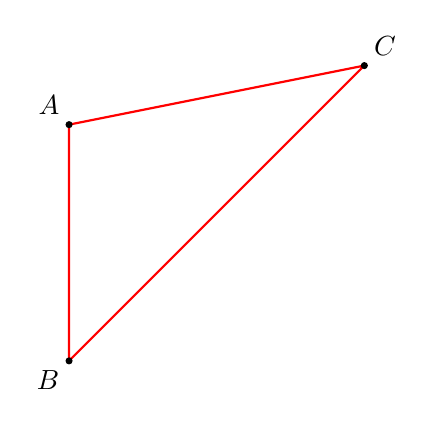
\begin{tikzpicture}[scale=0.75]
		\coordinate (A) at (-2,3);
		\coordinate (B) at (-2,-1);
		\coordinate (C) at (3,4);
		
		\tkzInit[xmin=-5,ymin=-5,xmax=5,ymax=5]
		\tkzGrid
		\tkzAxeXY
		
		% Triangle
		\draw[red, thick] (A) -- (B) -- (C) -- cycle;
		\filldraw (A) circle (0.05)
			node[above left]{$A$};
		\filldraw (B) circle (0.05)
			node[below left]{$B$};
		\filldraw (C) circle (0.05)
			node[above right]{$C$};
	\end{tikzpicture}
\end{center}

Per i primi due punti, questo è tutto quello che ci serve.\\
\textbf{Per il punto~\ref{enum:ex:retta:1:1}}, possiamo semplicemente usare la formula per la retta 
passante per due punti. Per convenienza, denominiamo le rette in base ai vertici che attraversano.\\
Per la retta $AB$ è immediato: si nota che hanno la stessa ascissa, quindi la retta passante per i due
punti è solo $\boxed{AB: x = -2}$.\\ [\baselineskip]
Per $AC$:
\begin{align*}
\frac{y-y_1}{y_2-y_1} = \frac{x-x_1}{x_2-x_1} &\rightarrow
\frac{y-3}{4-3} = \frac{x-(-2)}{3-(-2)} \rightarrow\\
\frac{y-3}{1} = \frac{x+2}{5} &\rightarrow y = \frac{x+2}{5} + 3\\
y = \frac{1}{5}x + \frac{2}{5} + \frac{15}{5} &\rightarrow \boxed{AC: y = \frac{1}{5}x + \frac{17}{5}}
\end{align*}
Infine per $BC$
\begin{align*}
\frac{y-y_1}{y_2-y_1} = \frac{x-x_1}{x_2-x_1} &\rightarrow
\frac{y+1}{4+1} = \frac{x-(-2)}{3+2}\\
\frac{y+1}{5} = \frac{x+2}{5} &\rightarrow \boxed{BC: y = x + 1}
\end{align*}

\textbf{Ci avviamo ora al punto~\ref{enum:ex:retta:1:2}} e per l'area possiamo usare la matrice
\begin{equation*}
\mathscr{A}(ABC) = \frac{1}{2}\left\lvert 
\begin{matrix}[1]
x_1 & y_1 & 1\\
x_2 & y_2 & 1\\
x_3 & y_3 & 1
\end{matrix}\right\rvert
\end{equation*}
Che poi si semplifica usando Sarrus in
\begin{equation*}
\mathscr{A}(ABC) = \frac{1}{2}\left\lvert x_1y_2 + y_1x_3 + x_2y_3 -x_3y_2 -y_3x_1 -x_2y_1\right\rvert
\end{equation*}
E sostituendo otteniamo
\begin{align*}
\mathscr{A}(ABC) &= \frac{1}{2}\left\lvert -2\cdot1 + 3\cdot3 -2\cdot4 -3\cdot1 - 4\cdot(-2) +
2\cdot3\right\rvert\\
\mathscr{A}(ABC) &= \frac{1}{2}\left\lvert -2+9-8-3+8+6\right\rvert\\
\Aboxed{\mathscr{A}(ABC) &= 10}
\end{align*}
Per trovare il perimetro, possiamo usare la distanza tra due punti e trovare tutte le lunghezze.\\
$AB$ è immediato in quanto hanno la stessa ascissa. $\boxed{AB = 3 + 1 = 4}$.\\ [\baselineskip]
Per trovare $AC$
\begin{align*}
AC &= \sqrt{(x_C-x_A)^2+(y_C-y_A)^2} \rightarrow \\
AB &= \sqrt{(3+2)^2 + (4-3)^2} = \sqrt{5^2+1^2} \\
 &= \sqrt{25+1} = \boxed{\sqrt{26}}
\end{align*}
Per trovare $BC$
\begin{align*}
BC &= \sqrt{(x_C-x_B)^2+(y_C-y_B)^2} \rightarrow \\
BC &= \sqrt{(3+2)^2+(4+1)^2} = \sqrt{5^2+5^2} =
\sqrt{25+25} \\
&= \sqrt{50} = \sqrt{5^2\cdot2} = \boxed{5\sqrt{2}}
\end{align*}
E ora non resta che sommare
\begin{equation*}
2p = AB + AC + BC = 4 + \sqrt{26} + 5\sqrt{2}
\end{equation*}

\textbf{Per il punto~\ref{enum:ex:retta:1:3}} aggiorniamo il disegno
\begin{center}
	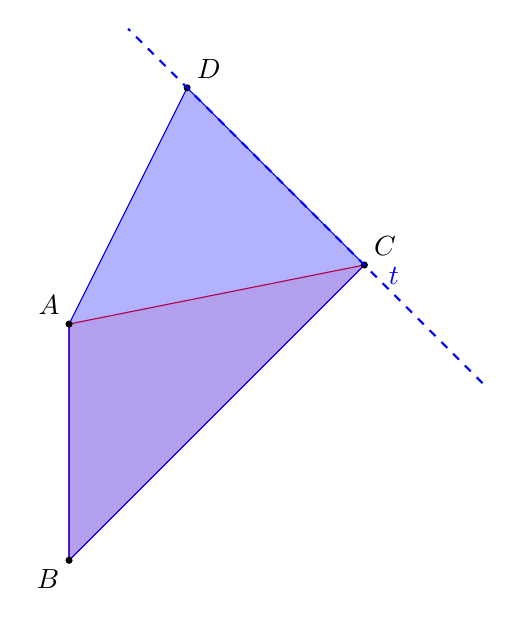
\begin{tikzpicture}[scale=0.75]
	\coordinate (A) at (-2,3);
	\coordinate (B) at (-2,-1);
	\coordinate (C) at (3,4);
	\coordinate (D) at (0,7);
	
	
	%\draw[step=1,very thin,darkgray] (-5,-3) grid (5,8);
	%\draw[thick,-stealth] (-5,0) -- (5,0)
	%	node[pos=1,above]{$x$};
	%\draw[thick,-stealth] (0,-3) -- (0,8)
	%	node[pos=1,right]{$y$};
	\tkzInit[xmax=5,ymax=8,xmin=-5,ymin=-3]
	\tkzGrid
	\tkzAxeXY
	
	\filldraw[red, fill opacity = 0.1](A) -- (B) -- (C) -- cycle;
	\filldraw[blue, fill opacity = 0.3] (A) -- (B) -- (C) -- (D) -- cycle;
	
	% Triangle
	\filldraw (A) circle (0.05)
		node[above left]{$A$};
	\filldraw (B) circle (0.05)
		node[below left]{$B$};
	\filldraw (C) circle (0.05)
		node[above right]{$C$};
	\filldraw (D) circle (0.05)
		node[above right]{$D$};
	
	\draw[dashed, blue, thick] (5,2) -- (-1,8)
		node[pos=0.25, above]{$t$};
	\end{tikzpicture}
\end{center}
Noi dobbiamo calcolare l'area di $ABCD$. Abbiamo varie strade che possiamo seguire. Ne propongo una
che può essere usata per praticamente ogni figura. Il tutto si basa su trovare l'area del rettangolo 
che contiene la figura e togliere dei triangoli che possiamo individuare. Nel nostro caso

\begin{center}
	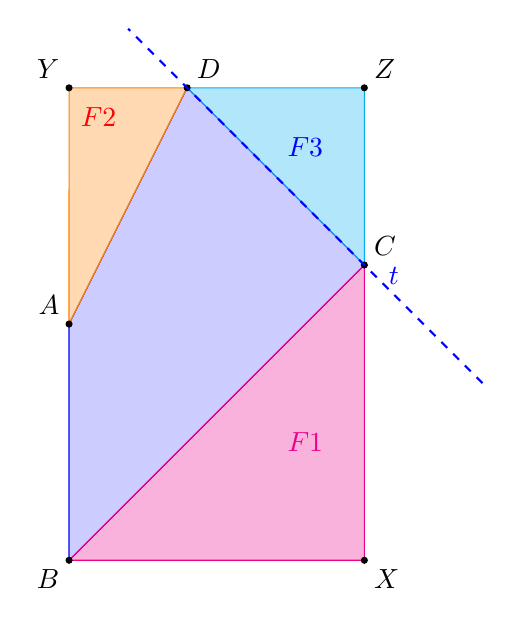
\begin{tikzpicture}[scale=0.75]
	\coordinate (A) at (-2,3);
	\coordinate (B) at (-2,-1);
	\coordinate (C) at (3,4);
	\coordinate (D) at (0,7);
	
	\tkzInit[xmin=-5,ymin=-3,xmax=5,ymax=8]
	\tkzGrid
	\tkzAxeXY
	
	%\filldraw[red, fill opacity = 0.1](A) -- (B) -- (C) -- cycle;
	\filldraw[blue, fill opacity = 0.2] (A) -- (B) -- (C) -- (D) -- cycle;
	\filldraw[magenta, fill opacity = 0.3] (B) -- (C) -- (3,-1) -- cycle;
	\filldraw[orange, fill opacity = 0.3] (A) -- (D) -- (-2,7) -- cycle;
	\filldraw[cyan, fill opacity = 0.3] (D) -- (C) -- (3,7) -- cycle;
	
	% Triangle
	\filldraw (A) circle (0.05)
		node[above left]{$A$};
	\filldraw (B) circle (0.05)
		node[below left]{$B$};
	\filldraw (C) circle (0.05)
		node[above right]{$C$};
	\filldraw (D) circle (0.05)
		node[above right]{$D$};
	\filldraw (3,-1)  circle (0.05)
		node[below right]{$X$};
	\filldraw (-2,7)  circle (0.05)
		node[above left]{$Y$};
	\filldraw (3,7) circle (0.05)
		node[above right]{$Z$};
	
	\draw[dashed, blue, thick] (5,2) -- (-1,8)
		node[pos=0.25, above]{$t$};
	\node[magenta] (F1) at (2,1){$F1$};
	\node[red] (F2) at (-1.5,6.5){$F2$};
	\node[blue] (F3) at (2,6){$F3$};
	\end{tikzpicture}
\end{center}

vediamo che possiamo trovare l'area facendo
\begin{equation*}
\mathscr{A}(YZXB) - \mathscr{A}(F1) - \mathscr{A}(F2) - \mathscr{A}(F3)
\end{equation*}
o più semplicemente, sostituendo
\begin{align*}
\mathscr{A}(ABCD) &= BX\cdot BY - \overbrace{\frac{5^2}{2}}^{\mathscr{A}(\mathcolor{magenta}{F1})} - 
\overbrace{\frac{2\cdot4}{2}}^{\mathscr{A}(\mathcolor{orange}{F2})} -
\overbrace{\frac{3^2}{2}}^{\mathscr{A}(\mathcolor{blue}{F3})} \\
&= 5\cdot8 - 12.5 - 4 -4.5 = 40 - 21 = 19
\end{align*}

Ora per \textbf{l'ultimo punto} possiamo semplificare il disegno e pulirlo un po'.
\begin{center}
	\begin{tikzpicture}[scale=0.75]
	
	\tkzInit[xmin=-5,ymin=-11,xmax=5,ymax=3]
	\tkzGrid
	\tkzAxeXY

	\draw[red, thick] (-2,-11) -- (-2,3);
	\draw[blue, thick] (-5,-10) -- (1.5,3)
		node[pos=0.75, right]{$y = 2x$};
	\filldraw (-5,-10) circle (0.05);
	\filldraw (1,2) circle (0.05);
	
	\draw[dashed, orange, very thick] (1,2) -- ++(-3,0);
	\draw[dashed, orange, very thick] (-5,-10) -- ++(3,0);
	\end{tikzpicture}
\end{center}

Per prima cosa dobbiamo trasformare in forma esplicita la retta $x = -2$ per poter usare la formula
della distanza Punto-Retta.
\begin{equation*}
r: x + 2 = 0
\end{equation*}
E ora possiamo scrivere la formula della distanza
\begin{align*}
d &= \frac{\left\lvert ax_P + by_P+c\right\rvert}{\sqrt{a^2+b^2}} \rightarrow
3 = \frac{\left\lvert x + 2\right\rvert}{\sqrt{1^2}} \\
3 &= \frac{\left\lvert x + 2\right\rvert}{\sqrt{1}} \rightarrow
3\cdot1 = \left\lvert x + 2\right\rvert\\
\pm3 &= x + 2 \rightarrow \begin{dcases}
x + 5 = 0\\
x - 1 = 0
\end{dcases} \rightarrow
\begin{dcases}
x = -5\\
x = 1
\end{dcases}
\end{align*}
Abbiamo le ascisse di intersezione con la retta $y = 2x$. Ora possiamo sostituire e trovare $y$.
\begin{equation*}
\begin{dcases}
y = -5\cdot2\\
y = 1\cdot2
\end{dcases} \rightarrow
\boxed{\begin{dcases}
P_1(-5,-10)\\
P_2(1,2)
\end{dcases}}
\end{equation*}

\subsubsection*{\hyperref[subsec:geomanal:fasciorette]{Fasci di rette}}
\paragraph{Esercizio 1}
Dopo aver verificato che l'equazione
\begin{equation*}
(2k+1)x -4ky + 3 + 2k = 0 \qquad (k\in\mathbb{R})
\end{equation*}
rappresenta un fascio proprio di rette, determinare:
\begin{enumerate}
	\item il centro $C$ del fascio; \label{enum:ex:retta:2:1}
	\item la retta $r_1$ del fascio perpendicolare alla bisettrice del $\ang{2}$ e $\ang{3}$ quadrante;
	detto $H$ il loro punto di incontro, trovare poi l'area del triangolo $CHO$, essendo $O$ l'orgine
	degli assi;\label{enum:ex:retta:2:2}
	\item le rette del fascio che intersecano il segmento $OH$;\label{enum:ex:retta:2:3}
	\item le bisettrici degli angoli formati dalle rette $CO$ e $CH$.\label{enum:ex:retta:2:4}
\end{enumerate}
\divisor

Prima di avere il disegno, dobbiamo avere qualcosa da disegnare. Se disegnassimo l'intero fascio 
sarebbe come colorare tutto il piano.\\
\textbf{Per il punto~\ref{enum:ex:retta:2:1}} dobbiamo mettere a sistema le due rette generatrici.
Nella forma attuale, le due equazioni non sono facilmente riconoscibili, quindi raccogliamo $k$ così
da isolare le due rette
\begin{align*}
(2k+1)x -4ky + 3 + 2k = 0 &\rightarrow 2kx+x-4ky+3+2k = 0 \rightarrow\\
k\underbrace{(2x-4y+2)}_{\text{Generatrice 1}}&+\underbrace{x+3}_{\text{Generatrice 2}} = 0
\end{align*}
Avendo ora questa forma, possiamo evidentemente vedere che effettivamente si tratta di un fascio 
proprio di rette.\\
Come trovare il centro del fascio? Avendo le due generatrici, le mettiamo a sistema e troviamo la loro
intersezione
\begin{align*}
\begin{dcases}
2x-4y+2=0\\
x=-3
\end{dcases} &\rightarrow
\begin{dcases}
-x-4y+2=0\\
x=-3
\end{dcases} \rightarrow\\
\begin{dcases}
\cancel{-4}y = \cancelto{-1}{4}\\
x=-3
\end{dcases} &\rightarrow
\boxed{\begin{dcases}
y = -1\\
x = -3
\end{dcases}}
\end{align*}

\textbf{Per il punto~\ref{enum:ex:retta:2:2}} facciamo il disegno
\begin{center}
	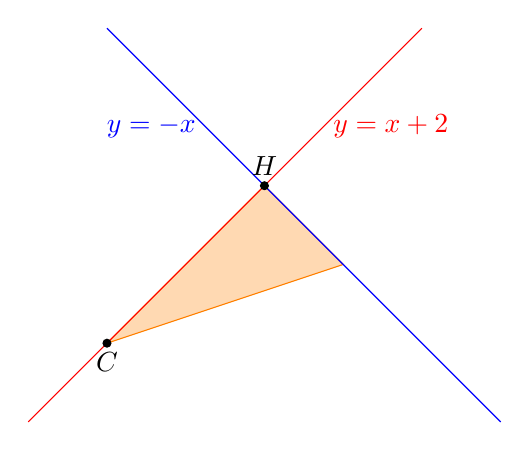
\begin{tikzpicture}
		\coordinate (C) at (-3,-1);
		\coordinate (H) at (-1,1);
		
		\tkzInit[xmin=-4,ymin=-2,xmax=3,ymax=3]
		\tkzGrid
		\tkzAxeXY
		
		\filldraw[orange, fill opacity = 0.3] (C) -- (H) -- (0,0) -- cycle;
		
		\draw[blue] (-3,3) -- (2,-2)
			node[pos=0.25, left]{$y = -x$};
		\draw[red] (-4,-2) -- (1,3)
			node[pos=0.75, right]{$y = x+2$};
			
		\filldraw (C) circle (0.05)
			node[below]{$C$};
		\filldraw (H) circle (0.05)
			node[above]{$H$};
	\end{tikzpicture}
\end{center}
Ho già inserito le cose che ora andiamo a trovare.\\
Innanzitutto sappiamo che la bisettrice del $\ang{2}$ e $\ang{3}$ quadrante è $y=-x$, quindi sappiamo
che la $m$ della perpendicolare deve essere uguale a $1$. Sappiamo anche che fa parte del fascio 
quindi passa per $C(-3,-1)$.
\begin{equation*}
y-y_0 = m(x-x_0) \rightarrow y+1 = x+3 \rightarrow \boxed{y = x+2}
\end{equation*}
E ora ci troviamo $H$, ovvero il punto di intersezione
\begin{equation*}
\begin{dcases}
y = x+2\\
y = -x
\end{dcases} \rightarrow
\begin{dcases}
-x = x+2\\
y = -x
\end{dcases} \rightarrow
\boxed{\begin{dcases}
x = -1\\
y = 1
\end{dcases}}
\end{equation*}
Ora possiamo trovare l'area del triangolo
\begin{align*}
\mathscr{A}(CHO) &= \frac{1}{2}\left\lvert x_1y_2 + y_1x_3 + x_2y_3 -x_3y_2 -y_3x_1-x_2y_1\right\rvert
\rightarrow\\
\mathscr{A}(CHO) &= \frac{1}{2}\left\lvert x_1y_2 + \cancel{y_1x_3} + \cancel{x_2y_3} 
-\cancel{x_3y_2} -\cancel{y_3x_1} -x_2y_1\right\rvert \rightarrow \\
\mathscr{A}(CHO) &= \frac{1}{2}\left\lvert x_1y_2 -x_2y_1\right\rvert \rightarrow
\mathscr{A}(CHO) = \frac{1}{2}\left\lvert -3 -1\right\rvert =\\
\frac{1}{2}&\left\lvert-4\right\rvert \rightarrow \mathscr{A}(CHO) = \frac{1}{2}\cdot4 = \boxed{2}
\end{align*}

\textbf{Il punto~\ref{enum:ex:retta:2:3}}, richiede di trovare i $k$ per cui una retta del fascio 
passi in mezzo al segmento $OH$. La prima cosa da fare è quindi trovare i $k$ degli "estremi" $O$ e
$H$.
\begin{equation*}
k_O = -\frac{a_1x_O+b_1y_O+c_1}{ax_O+by_O+c} \rightarrow k_O = -\frac{c_1}{c} = -\frac{3}{2}
\end{equation*}
\begin{equation*}
k_H = -\frac{a_1x_H+b_1y_H+c_1}{ax_H+by_H+c} \rightarrow k_H = -\frac{-1+0+3}{-2-4+2} = \frac{1}{2}
\end{equation*}

Ora sapendo che la retta esclusa attraversa anch'essa il segmento (per dimostrarlo basta 
semplicemente disegnarla), deduciamo che ai lati della esclusa ci siano le rette per $k\to\pm\infty$,
ovvero man mano che ci si avvicina alla retta esclusa più ci si avvicina all'infinito. Questo ci porta
a trovare l'intervallo che è
\begin{equation*}
\boxed{k\leq-\frac{3}{2} \vee k\geq\frac{1}{2}}
\end{equation*}

Infine, il \textbf{punto~\ref{enum:ex:retta:2:4}} richiede un po' di ragionamento. Una bisettrice è la
retta passante per due punti equidistanti alle rette dell'angolo. Per prima cosa quindi, definiamo
$P(x,y)$ un punto del piano in modo che sia $d_{P,CO} = d_{P,CH}$. Per prima cosa dunque dobbiamo 
trovare le rette che passano per $CO$ e $CH$.
\begin{align*}
\frac{y-y_1}{y_2-y_1} &= \frac{x-x_1}{x_2-x_1} \rightarrow
\frac{y+1}{1+1} = \frac{x+3}{-1+3} \rightarrow\\
y+1 &= x+3 \rightarrow CO:\, x-y+2 = 0
\end{align*}
\begin{align*}
\frac{y-y_1}{y_2-y_1} &= \frac{x-x_1}{x_2-x_1} \rightarrow
\frac{y+1}{1}= \frac{x+3}{3} \rightarrow\\
3y+3 &= x+3 \rightarrow CH:\, -x+3y=0
\end{align*}
E ora possiamo scrivere le formule per le distanze
\begin{align*}
\frac{\lvert x-y+2\rvert}{1} = \frac{\lvert -x+3y\rvert}{\sqrt{10}} &\rightarrow\\
\sqrt{10}(\lvert x-y+2\rvert) = \lvert -x+3y\rvert &\rightarrow\\
\sqrt{10}x-\sqrt{10}y+2\sqrt{10} = \pm(-x+3y) &\rightarrow\\
\begin{cases}
\sqrt{10}x-\sqrt{10}y+2\sqrt{10} = -x+3y\\
\sqrt{10}x-\sqrt{10}y+2\sqrt{10} = x-3y
\end{cases} &\rightarrow\\
\begin{cases}
x(\sqrt{10}+1)-y(\sqrt{10}+3) + 2\sqrt{10}\\
x(\sqrt{10}-1)-y(\sqrt{10}-3) + 2\sqrt{10}
\end{cases} &\rightarrow\\
\boxed{x(\sqrt{10}\pm1)-y(\sqrt{10}\pm3)+2\sqrt{10}}
\end{align*}

\subsubsection*{\hyperref[subsec:geomana:circ]{Circonferanza}}\label{ex:circ}
\paragraph{Esercizio 1}
Determinare l'equazione della circonferenza passante per $A(-2,2)$ e $B(4,-4)$ e avente il centro
sulla retta $x+2y-8=0$, e le equazioni delle rette $t_1$ e $t_2$ passanti per $H(0,8)$ e tangenti 
alla circonferenza. detta poi $t_1$ la tangente con coefficiente angolare positivo, determinare le
rette ad essa perpendicolari che formano con gli assi cartesiani un triangolo di area 
$\dfrac{54}{5}$. Determinare, inoltre, i punti di $t_1$ che hanno distanza uguale a $\sqrt{2}$ dal
la retta $x+y-1=0$.
\divisor

Per prima cosa dobbiamo trovare l'equazione della circonferenza $\mathscr{C}$. Come fare? Sappiamo che
$A$ e $B$ appartengono alla circonferenza e che il centro appartiene a $x+2y-8=0$. Mettiamo queste
informazioni a sistema e risolviamo
\begin{align*}
&\begin{dcases}
4+4-2a+2b+c=0\\
16+16+4a-4b+c=0\\
-\frac{a}{2}-b-8=0
\end{dcases}\rightarrow\\
&\begin{dcases}
-8+2a-2b=c\\
32+4a-4b-8+2a-2b=0\\
-\frac{a}{2}-b-8=0
\end{dcases}\rightarrow\\
&\begin{dcases}
-8+2a-2b=c\\
\cancelto{4}{24}+\cancelto{1}{6}a-\cancelto{1}{6}b=0\\
-\frac{a}{2}-b-8=0
\end{dcases}\rightarrow
\begin{dcases}
-8+2a-2b=c\\
4+a+\frac{a}{2}+8=0\\
b=-\frac{a}{2}-8
\end{dcases}\rightarrow\\
&\begin{dcases}
-8+2a-2b=c\\
\frac{\cancel{3}}{\cancel{2}}a = -\cancelto{8}{12}\\
b = -\frac{a}{2}-8
\end{dcases}\rightarrow
\begin{dcases}
\cancel{-8}-16\cancel{+8}=c\\
a = -8\\
b = -\frac{8}{2}-8
\end{dcases}\rightarrow\\
&\begin{dcases}
c = -16\\
a = -8\\
b = -4
\end{dcases} \rightarrow \boxed{\mathscr{C}:\,x^2+y^2-8x-4y-16=0}
\end{align*}
Avendo ora l'equazione possiamo disegnarla.
\begin{center}
	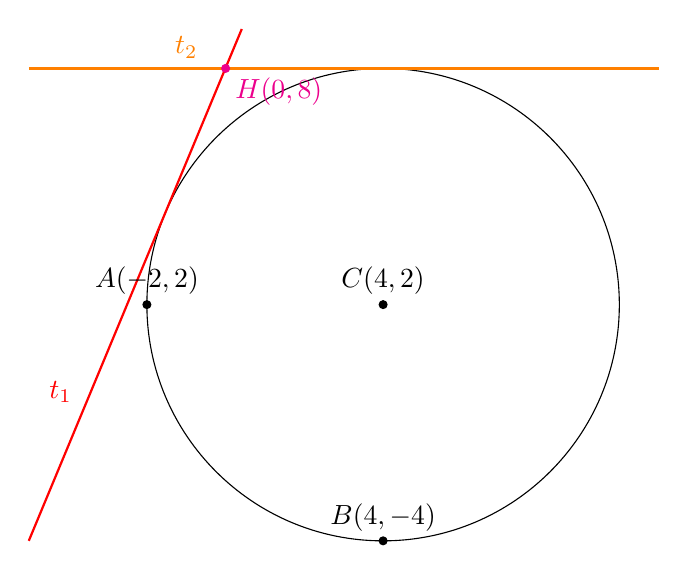
\begin{tikzpicture}[scale=0.5]
		\coordinate (C) at (4,2);
		\coordinate (A) at (-2,2);
		\coordinate (B) at (4,-4);
		\coordinate (H) at (0,8);
		\def\R{6};
		
		\tkzInit[xmin=-5,ymin=-5,xmax=11,ymax=9]
		\tkzGrid
		\tkzAxeXY
		
		\draw (C) circle(\R);
		\draw[orange, thick] (-5,8) -- (11,8)
			node[pos=0.25,above]{$t_2$};
		\draw[red,thick] (-5,-4) -- (0.41,9)
			node[pos=0.25,above left]{$t_1$};
		
		\filldraw (C) circle (0.1)
			node[above]{$C(4,2)$};
		\filldraw (A) circle (0.1)
			node[above]{$A(-2,2)$};
		\filldraw (B) circle (0.1)
			node[above]{$B(4,-4)$};
		\filldraw[magenta] (H) circle (0.1)
			node[below right]{$H(0,8)$};
	\end{tikzpicture}
\end{center}
Per trovare le due tangenti alla circonferenza che passano per $H$, ci troviamo il fascio di rette 
che ha $H$ come centro
\begin{equation*}
y-y_0=m(x-x_0) \rightarrow y-mx-8=0
\end{equation*}
e sappiamo che le tangenti hanno il loro punto di tangenza che dista dal centro esattamente $r$, 
quindi
\begin{align*}
\frac{\lvert ax_P + y_P + c_P\rvert}{\sqrt{a^2+b^2}} = d &\rightarrow
\frac{\lvert-4m+2-8\rvert}{\sqrt{1^2+m^2}} = 6 \rightarrow\\
\lvert-4m+2-8\rvert^2 &= (6\sqrt{1^2+m^2}) \rightarrow\\
16m^2\cancel{+36}+48m&=\cancel{36} + 36m^2 \rightarrow\\
\cancelto{-5}{-20}m^2+\cancelto{12}{48}m = 0 &\rightarrow 5m^2-12m =0 \\
m_{1/2} = \frac{12\pm\sqrt{144+0}}{10} &\rightarrow \boxed{\begin{dcases}
m_1 = \frac{12}{5}\\
m_2 = 0
\end{dcases}}
\end{align*}
e le tangenti sono
\begin{equation*}
\boxed{t_1:\,y = \frac{12}{5}x+8 \qquad t_2:\, y=8}
\end{equation*}

Ora dobbiamo trovare tutte le perpendicolari a $t_1$ che, con l'interesezione degli assi forma un
triangolo di area $\dfrac{54}{5}$. Per farlo, intanto troviamo le perpendicolari.
\begin{equation*}
\mathscr{F_\perp}:\,y=-\frac{5}{12}x + q
\end{equation*}
E ora possiamo trovare le intersezioni con gli assi
\begin{equation*}
\begin{dcases}
x = 0\\
y = q
\end{dcases}\qquad
\begin{dcases}
x = -\frac{12}{5}q\\
y = 0
\end{dcases}
\end{equation*}

E ora imponiamo che l'area del triangolo formato con gli assi sia uguale a $\dfrac{54}{5}$
\begin{equation*}
\frac{54}{5} = \frac{1}{2}\left\lvert q\cdot-\frac{12}{5}q\right\rvert \rightarrow
\frac{54}{5} = \frac{6}{5}\lvert q^2\rvert \rightarrow 9 = q^2 \rightarrow q = \pm3
\end{equation*}
quindi le rette cercate sono
\begin{equation*}
\boxed{y = -\frac{5}{12}x\pm3}
\end{equation*}

Finalmente possiamo avviarci alla conclusione. Dobbiamo cercare i punti di $t_1$ che distano 
$\sqrt{2}$ da $x+y-1$. Per prima cosa quindi, troviamo le rette che distano $\sqrt{2}$ dalla data
\begin{align*}
\frac{\lvert x+y-1\rvert}{\sqrt{2}} = \sqrt{2} \rightarrow \lvert x+y-1\rvert = 2 \rightarrow\\
\begin{cases}
x+y-1=2\\
x+y-1=-2
\end{cases} \rightarrow
\begin{cases}
x+y-3=0\\
x+y+1=0
\end{cases}
\end{align*}
e ora non resta che trovare le intersezioni con $t_1$
\begin{equation*}
\begin{dcases}
x+y+1=0\\
y=\frac{12}{5}x+8
\end{dcases}\rightarrow
\begin{dcases}
x+\frac{12}{5}x+8+1=0\\
y=\frac{12}{5}x+8
\end{dcases}\rightarrow
\boxed{\begin{dcases}
x = -\frac{45}{17}\\
y = \frac{76}{17}
\end{dcases}}
\end{equation*}
\begin{equation*}
\begin{dcases}
x+y-3=0\\
y=\frac{12}{5}x+8
\end{dcases}\rightarrow
\begin{dcases}
x+\frac{12}{5}x+5=0\\
y=\frac{12}{5}x+8
\end{dcases}\rightarrow
\boxed{\begin{dcases}
x = -\frac{25}{17}\\
y = \frac{76}{17}
\end{dcases}}
\end{equation*}

\subsubsection*{\hyperref[subsec:geomanal:fasciocirc]{Fasci di circonferenze}}
\paragraph{Esecizio 1}
Avendo il fascio
\begin{equation*}
x^2+y^2-2(k+1)x-2ky-4k+1=0
\end{equation*}
indicare con $\gamma_1$ quella il cui centro $C$ appartiene
alla retta $3x-y+5=0$. Detti $E$ ed $F$ i punti di intersezione di $\gamma_1$ con l'asse $y$, trovare
le equazioni delle tangenti a $\gamma_1$ in $E$ ed $F$; detto inoltre $T$ il loro punto di 
intersezione, dopo aver dimostrato che il quadrilatero $CETF$ è un quadrato, calcolarne l'area. 
Determinare inoltre l'equazione della circonfereza d centro $T$ e tangente esternamente a $\gamma_1$.
\divisor

Per prima cosa riordiniamo l'equazione per avere tutti i coefficienti
\begin{align*}
x^2+y^2-2(k+1)x-2ky-4k+1=0 \rightarrow\\
x^2+y^2+x(-2k-2)+y(-2k)+4k+1=0
\end{align*}
avendo ora i coefficienti, possiamo imporre la condizione che il centro sia un punto della retta
\begin{align*}
&3\left(-\frac{a}{2}\right)-\left(-\frac{b}{2}\right)-5=0 \rightarrow
3\frac{2k+2}{2}-k-5=0 \rightarrow\\ &6k+6-2k-10=0\rightarrow k=1
\end{align*}
e sostituire per ottenere
\begin{equation*}
\boxed{\gamma_1:\, x^2+y^2-4x-2y-3=0}
\end{equation*}
Prima di proseguire, disegnamo la circonferenza
\begin{center}
	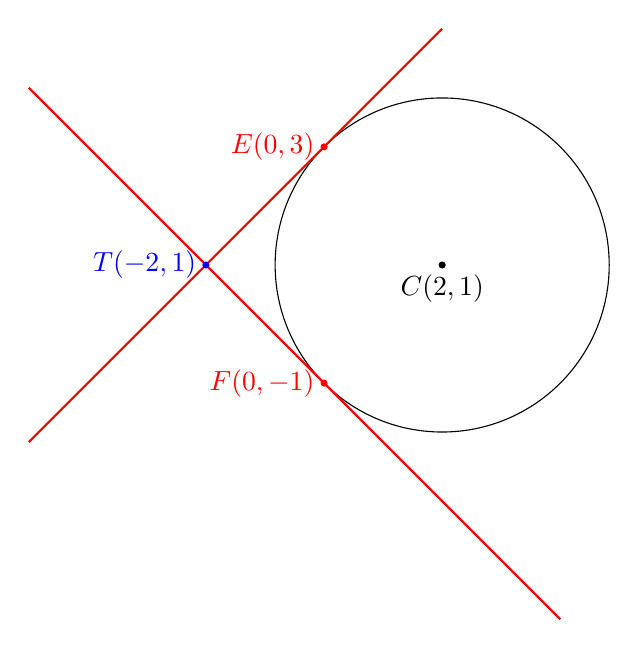
\begin{tikzpicture}[scale=0.75]
		\coordinate (C) at (2,1);
		\coordinate (E) at (0,3);
		\coordinate (F) at (0,-1);
		\coordinate (T) at (-2,1);
		\def\R{2.8284};
		
		\tkzInit[xmin=-5,ymin=-5,xmax=5,ymax=5]
		\tkzGrid
		\tkzAxeXY
		
		\draw (C) circle(\R);
		\draw[thick, red, domain=-5:2] plot(\x,\x+3);
		\draw[thick,red, domain=-5:4] plot(\x,-\x-1);
		
		\filldraw (C) circle (0.05)
			node[below]{$C(2,1)$};
		\filldraw[red] (E) circle (0.05)
			node[left]{$E(0,3)$};
		\filldraw[red] (F) circle (0.05)
			node[left]{$F(0,-1)$};
		\filldraw[blue] (T) circle (0.05)
			node[left]{$T(-2,1)$};
	\end{tikzpicture}
\end{center}
Sono già segnati i punti che ora andremo a trovare: $E$ e $F$ ovvero le intersezioni con $y$.
\begin{equation*}
y^2-2y-3=0\rightarrow
y_{1/2} = \frac{2\pm\sqrt{4+12}}{2} = \frac{2\pm4}{2} \rightarrow \begin{cases}
y_1 = 3\\
y_2 = -1
\end{cases}
\end{equation*}
Quindi i due punti sono
\begin{equation*}
\boxed{E(0,3)\qquad F(0,-1)}
\end{equation*}

Ora troviamo le tangenti in $E$ ed $F$.
\begin{align*}
&x\cdot x_P+y\cdot y_P+a\frac{x+x_P}{2}+b\frac{y+y_P}{2}+c = 0\rightarrow\\
&t_E:\, x\cdot0+y\cdot3-4\frac{x+0}{2}-2\frac{y+3}{2}-3=0 \rightarrow\\
&\boxed{-x+y-3=0 \rightarrow y = x+3}
\end{align*}
e
\begin{align*}
&x\cdot x_P+y\cdot y_P+a\frac{x+x_P}{2}+b\frac{y+y_P}{2}+c = 0\rightarrow\\
&t_F:\, x\cdot0+y\cdot(-1)-4\frac{x+0}{2}-2\frac{y-1}{2}-3=0\rightarrow\\
&\boxed{-x-y-1=0\rightarrow y=-x-1}
\end{align*}
E ora possiamo trovare il punto di intersezione
\begin{align*}
\begin{cases}
y=x+3\\
y=-x-1
\end{cases}\rightarrow
\begin{cases}
-x-1=x+3\\
y=-x-1
\end{cases}\rightarrow
\begin{cases}
x = -2\\
y=1
\end{cases}
\end{align*}
Aggiorniamo ora il disegno per mettere in luce il quadrato $CETF$
\begin{center}
	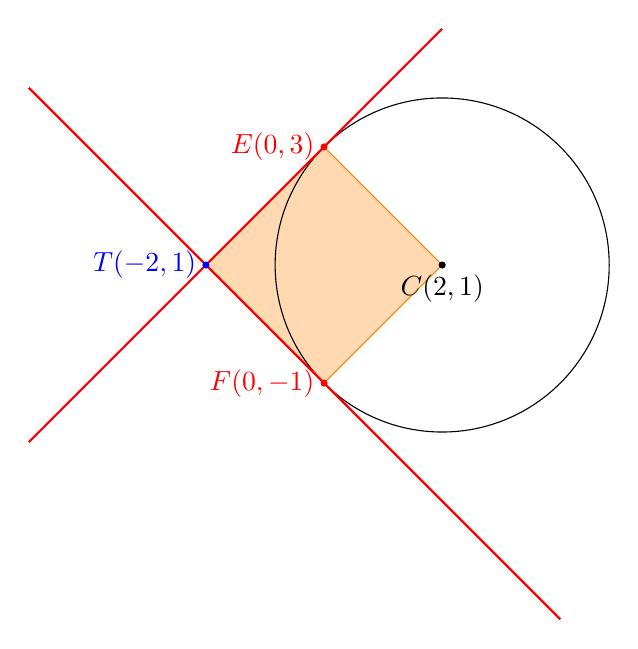
\begin{tikzpicture}[scale=0.75]
	\coordinate (C) at (2,1);
	\coordinate (E) at (0,3);
	\coordinate (F) at (0,-1);
	\coordinate (T) at (-2,1);
	\def\R{2.8284};
	
	\tkzInit[xmin=-5,ymin=-5,xmax=5,ymax=5]
	\tkzGrid
	\tkzAxeXY
	
	\filldraw[orange, fill opacity=0.3] (C) -- (E) -- (T) -- (F) -- cycle;
		
	\draw (C) circle(\R);
	\draw[thick, red, domain=-5:2] plot(\x,\x+3);
	\draw[thick,red, domain=-5:4] plot(\x,-\x-1);
	
	\filldraw (C) circle (0.05)
	node[below]{$C(2,1)$};
	\filldraw[red] (E) circle (0.05)
	node[left]{$E(0,3)$};
	\filldraw[red] (F) circle (0.05)
	node[left]{$F(0,-1)$};
	\filldraw[blue] (T) circle (0.05)
	node[left]{$T(-2,1)$};
	\end{tikzpicture}
\end{center}

Come possiamo dimostrare che è un quadrato? Proviamo a guardare gli angoli: l'angolo $C\widehat{F}T$
e l'angolo $C\widehat{E}T$ sono sicuramente retti in quanto sono angoli formati da un raggio e una 
tangente e per definizione stessa di tangente sono retti. Anche l'angolo $F\widehat{T}E$ è retto in
quanto i coefficienti angolari delle tangenti sono reciprocamente opposti ($m_1m_2=-1$). Ora manca
solo l'angolo $E\widehat{C}F$ da dimostrare. Possiamo semplicemente guardare il coefficiente angolare
della retta che passa tra $F$ e $C$ e vedere che risulta pari a 
\begin{equation*}
m = \frac{y_2-y_1}{x_2-x_1} \rightarrow m= \frac{1+1}{2-0} = 1
\end{equation*}
che è esattamente uguale a quello di $t_E$ quindi le due rette sono parallele. Se $t_F$ incide su 
$t_E$ con un angolo retto, deve per forza incidere con lo stesso angolo anche nelle sue parallele.\\
Abbiamo dimostrato che ha quattro angoli retti, per dimostrare che è un quadrato basta vedere che due
dei lati (che formano un angolo retto) sono uguali in quanto sono raggi. Quindi $CETF$ è un 
quadrato.\\
Per trovarne l'area basta elevare alla seconda la lunghezza del raggio
\begin{equation*}
r = \sqrt{x_C^2+y_C^2-c} \rightarrow r = \sqrt{8} = 2\sqrt{2}
\end{equation*}
E quindi l'area vale
\begin{equation*}
\mathscr{A}(CETF) = r^2 \rightarrow \mathscr{A}(CETF) = \sqrt{8}^2 = 8
\end{equation*}

Infine dobbiamo trovare la circonferenza con centro $T$ e tangente esternamente a $\gamma_1$. Per 
farlo abbiamo molti modi, ecco il più semplice. Sappiamo già quanto deve valere il raggio perché 
tocchi la circonferenza. Deve essere pari a $TC-r_{\gamma_1}$. Quindi
\begin{equation*}
r = TC-r_{\gamma_1} \rightarrow r = 4-2\sqrt{2}
\end{equation*}

Usando la formula per trovare il raggio possiamo scrivere
\begin{equation*}
r = \sqrt{\frac{a^2}{4}+\frac{b^2}{4}-c} \rightarrow 
4-2\sqrt{2} = \sqrt{\frac{a^2}{4}+\frac{b^2}{4}-c}
\end{equation*}
Abbiamo 3 variaibli quindi dobbiamo trovare un modo per toglierne 2. $a$ e $b$ sono utilizzate anche 
nella formula per trovare il centro della circonferenza. Si da il caso che noi abbiamo il centro!
Quindi
\begin{equation*}
\begin{dcases}
-\frac{a}{2} = -2\\
-\frac{b}{2} = 1
\end{dcases}\rightarrow
\begin{dcases}
a=4\\
b=-2
\end{dcases}
\end{equation*}
e ora possiamo trovare $c$
\begin{align*}
4-2\sqrt{2} = \sqrt{\frac{a^2}{4}+\frac{b^2}{4}-c} &\rightarrow 
4-2\sqrt{2} = \sqrt{\frac{16}{4}+\frac{4}{4}-c} \rightarrow\\
4-2\sqrt{2} = \sqrt{5-c} &\rightarrow
24-16\sqrt{2} = 5-c \rightarrow\\
c &= 16\sqrt{2}-19
\end{align*}
Quindi la nostra circonferenza sarà
\begin{equation*}
\boxed{\gamma:\, x^2+y^2+4x-2y+16\sqrt{2}-19=0}
\end{equation*}

\subsubsection*{\hyperref[subsec:geomanal:parabola]{Parabola}}\label{ex:parabola}
\paragraph{Esercizio 1}
Nel piano $xOy$ determinare
\begin{enumerate}
	\item l'equazione della parabola $\mathscr{P}_1$ avente asse parallelo all'asse $y$ e passante per
	$A(2,0)$, $B(6,0)$ e $C(0,6)$;\label{enum:ex:parabola:1:1}
	\item l'area del triangolo $ACH$ essendo $H$ l'ulteriore punto di intersezione di $\mathscr{P}_1$
	con la perpendicolare per $A$ alla retta $AC$;\label{enum:ex:parabola:1:2}
	\item l'equazione della circonferenza circoscritta al triangolo $CAH$;\label{enum:ex:parabola:1:3}
\end{enumerate}
\divisor

Per trovare l'equazione della parabola, possiamo sfruttare i 3 punti conosciuti e metterli a sistema
\begin{align*}
&\begin{cases}
4a+2b+c=0\\
36a+6b+c=0\\
c=6
\end{cases}\rightarrow
\begin{dcases}
a = \frac{-b-3}{2}\\
\cancelto{18}{36}\frac{-b-3}{\cancel{2}}+6b+6=0\\
c=6
\end{dcases}\rightarrow\\
&\begin{dcases}
a = \frac{-b-3}{2}\\
-18b-54_6b+6=0\\
c=6
\end{dcases}\rightarrow
\begin{dcases}
a = \frac{1}{2}\\
b = -4\\
c = 6
\end{dcases} \rightarrow\\ &\boxed{\mathscr{P}_1:\,y=\frac{1}{2}x^2-4x+6}
\end{align*}

E per concludere il punto~\ref{enum:ex:parabola:1:1} disegnamo il grafico
\begin{center}
	\begin{tikzpicture}[scale=0.75]
		\coordinate (A) at (2,0);
		\coordinate (B) at (6,0);
		\coordinate (C) at (0,6);
		\coordinate (H) at (20/3,14/9);
		
		%\filldraw[orange, fill opacity = 0.3] (A) -- (H) -- (C) -- cycle;
		
		\tkzInit[xmin=-1,ymin=-2,xmax=9,ymax=7]
		\tkzGrid
		\tkzAxeXY
		
		\draw[thick, domain=-0.25:8.25] plot(\x, {0.5*\x*\x-4*\x+6});
		%\draw[red, domain=-0.3:2.7] plot(\x,{-3*\x+6});
		%\draw[red, thick, domain=-1:9] plot(\x, {\x/3-2/3});
		
		\filldraw (A) circle (0.05)
			node[below]{$A(2,0)$};
		\filldraw (B) circle (0.05)
			node[below]{$B(6,0)$};
		\filldraw (C) circle (0.05)
			node[below]{$C(0,6)$};
		%\filldraw (H) circle (0.05)
			%node[right]{$H(\dfrac{20}{3},\dfrac{14}{9})$};
	\end{tikzpicture}
\end{center}

Il punto~\ref{enum:ex:parabola:1:2} richiede qualche passaggio intermedio. Per prima cosa troviamo
la retta passante per $AC$
\begin{equation*}
r_{AC}:\, \frac{y-y_1}{y_2-y_1} = \frac{x-x_1}{x_2-x_1} \rightarrow \frac{y}{6}=\frac{x-2}{-2}
\rightarrow r_{AC}:\,y=-3x+6
\end{equation*}

E ora dobbiamo trovare la perpendicolare passante per $A$.
\begin{align*}
r_{\perp AH}&:\,y=-\frac{1}{m}x+q \rightarrow y=\frac{x}{3}+q\rightarrow 0=\frac{2}{3}+q \rightarrow\\
r_{\perp AH}&:\,y=\frac{x}{3}-\frac{2}{3}
\end{align*}

E possiamo trovare $H$ facendo l'intersezione con la parabola $\mathscr{P}_1$
\begin{align*}
&\begin{dcases}
y = \frac{1}{2}x^2-4x+6\\
y=\frac{x}{3}-\frac{2}{3}
\end{dcases}\rightarrow
\begin{dcases}
\frac{x}{3}-\frac{2}{3} = \frac{1}{2}x^2-4x+6\\
y=\frac{x}{3}-\frac{2}{3}
\end{dcases}\rightarrow\\
&-\frac{1}{2}x^2+\frac{13}{3}x-\frac{20}{3}=0 \rightarrow 
x_{1/2} = \\
&\frac{-\frac{13}{3}\pm\sqrt{\frac{169}{9}-4\cdot-\frac{1}{2}\cdot-\frac{20}{3}}}{-1} 
\rightarrow\\ &-\frac{13}{3}\pm\frac{7}{3}\rightarrow\begin{dcases}
x_1 = 2\\
x_2 = \frac{20}{3}
\end{dcases}
\end{align*}
Il primo risultato ce lo aspettavamo in quanto è il punto $A$ che fa parte sia della retta che della
parabola.
\begin{equation*}
y = \frac{1}{2}x^2-4x+6 \, \text{con } x = \frac{20}{3} \rightarrow y = \frac{14}{9}
\end{equation*}
E quindi il nostro punto è
\begin{equation*}
H\left(\frac{20}{3},\frac{14}{9}\right)
\end{equation*}
Prima di proseguire, aggiorniamo il disegno
\begin{center}
	\begin{tikzpicture}[scale=0.75]
	\coordinate (A) at (2,0);
	\coordinate (B) at (6,0);
	\coordinate (C) at (0,6);
	\coordinate (H) at (20/3,14/9);
	\coordinate (M) at (1,3);
	\coordinate (N) at (13/3,7/9);
	\coordinate (K) at (10/3,34/9);
	
	\tkzInit[xmin=-1,ymin=-2,xmax=9,ymax=7]
	\tkzGrid
	\tkzAxeXY
	
	\filldraw[orange, fill opacity = 0.3] (A) -- (H) -- (C) -- cycle;
	
	\draw[thick, domain=-0.25:8.25] plot(\x, {0.5*\x*\x-4*\x+6});
	\draw[red, domain=-0.3:2.7] plot(\x,{-3*\x+6});
	\draw[red, thick, domain=-1:9] plot(\x, {\x/3-2/3});
	%\draw[blue, thick, domain=-1:9] plot(\x, {1/3*\x+8/3}); % M
	%\draw[blue, thick, domain=2.25:5.25] plot(\x, {-3*\x+124/9}); % N
	%\draw[blue, thick, domain=-0.5:5.5] plot(\x, {3/2*\x-11/9}); % K
	
	\filldraw (A) circle (0.05)
	node[below]{$A(2,0)$};
	\filldraw (B) circle (0.05)
	node[below]{$B(6,0)$};
	\filldraw (C) circle (0.05)
	node[below]{$C(0,6)$};
	\filldraw (H) circle (0.05)
	node[right]{$H(\dfrac{20}{3},\dfrac{14}{9})$};
	%\filldraw (M) circle (0.05)
	%node[above]{$M$};
	%\filldraw (K) circle (0.05)
	%node[above]{$K$};
	%\filldraw (N) circle (0.05)
	%node[above]{$N$};
	\end{tikzpicture}
\end{center}
L'area del triangolo è facilmente calcolabile con la formula
\begin{equation*}
\mathscr{A}(\mathscr{T}) = \frac{1}{2}\lvert
x_1y_2+y_1x_3+x_2y_3
-x_3y_2-y_3x_1-x_2y_1
\rvert
\end{equation*}
e quindi sostituendo
\begin{align*}
\mathscr{A}(\mathscr{T}) &= \frac{1}{2}\lvert
\cancel{x_1y_2}+y_1x_3+x_2y_3
\cancel{-x_3y_2}\cancel{-y_3x_1}-x_2y_1
\rvert \rightarrow\\
\mathscr{A}(\mathscr{T}) &= \frac{1}{2}\lvert 6\frac{20}{3}+2\frac{14}{9}-2\cdot6\rvert  = 
\frac{1}{2}\frac{280}{9} = \boxed{\frac{140}{9}}
\end{align*}

Il punto~\ref{enum:ex:parabola:1:3} richiede qualche passaggio intermedio anch'esso. Per trovare la
circonferenza circoscritta al triangolo, dobbiamo innanzitutto trovare il centro. In un triangolo 
qualsiasi, il centro della circonferenza circoscritta è denominato \emph{circocentro} ed esso è il
punto di intersezione degli assi dei lati. Quindi per prima cosa si trovino i punti medi dei lati
utilizzando la formula
\begin{equation*}
\left(\frac{x_1+x_2}{2},\frac{y_1+y_2}{2}\right)
\end{equation*}
e otteniamo i seguenti risultati
\begin{equation*}
M(1,3) \qquad N\left(\frac{13}{3},\frac{7}{9}\right) \qquad K\left(\frac{10}{3},\frac{34}{9}\right)
\end{equation*}

Dobbiamo poi trovarci le rette dei lati per poi poter trovarne le perpendicolari. Avendo già fatto
il processo, riporto solo i risultati
\begin{align*}
r_{AC}&:\,y=-3x+6\\
r_{CH}&:\,y=-\frac{2}{3}x+6\\
r_{AH}&:\,y=\frac{x}{3}-\frac{2}{3}
\end{align*}
Per trovare le perpendicolari abbiamo una formula molto comoda
\begin{equation*}
y = -\frac{1}{m}(x-x_0)+mx_0+q
\end{equation*}
Essendo anche qui solo una questione di calcoli, riporto solo i risultati
\begin{align*}
r_{\perp AC}&:\,y=\frac{1}{3}x+\frac{8}{3}\\
r_{\perp CH}&:\,y=\frac{3}{2}x+\frac{65}{9}\\
r_{\perp AH}&:\,y=-3x+\frac{124}{9}
\end{align*}
E ora possiamo disegnare
\begin{center}
	\begin{tikzpicture}[scale=0.75]
	\coordinate (A) at (2,0);
	\coordinate (B) at (6,0);
	\coordinate (C) at (0,6);
	\coordinate (H) at (20/3,14/9);
	\coordinate (M) at (1,3);
	\coordinate (N) at (13/3,7/9);
	\coordinate (K) at (10/3,34/9);
	
	\def\R{4};
	
	\tkzInit[xmin=-1,ymin=-2,xmax=9,ymax=8]
	\tkzGrid
	\tkzAxeXY
	
	\filldraw[orange, fill opacity = 0.3] (A) -- (H) -- (C) -- cycle;
	
	\draw[thick, domain=-0.45:8.45] plot(\x, {0.5*\x*\x-4*\x+6});
	\draw[red, domain=-0.65:2.7] plot(\x,{-3*\x+6});
	\draw[red, thick, domain=-1:9] plot(\x, {\x/3-2/3});
	\draw[blue, domain=-1:9] plot(\x, {1/3*\x+8/3}); % M
	\draw[blue, domain=1.95:5.25] plot(\x, {-3*\x+124/9}); % N
	\draw[blue, domain=-0.5:6.15] plot(\x, {3/2*\x-11/9}); % K
	\draw[thick] (K) circle (\R);
	
	\filldraw (A) circle (0.05)
	node[below]{$A(2,0)$};
	\filldraw (B) circle (0.05)
	node[below]{$B(6,0)$};
	\filldraw (C) circle (0.05)
	node[below]{$C(0,6)$};
	\filldraw (H) circle (0.05)
	node[right]{$H(\dfrac{20}{3},\dfrac{14}{9})$};
	\filldraw (M) circle (0.05)
	node[above]{$M$};
	\filldraw (K) circle (0.05)
	node[above]{$K$};
	\filldraw (N) circle (0.05)
	node[above]{$N$};
	\end{tikzpicture}
\end{center}
Da questo disegno possiamo vedere che il punto di intersezione tra le tre rette è esattamente $K$.
Quindi per definire la circonferenza, basta solo trovare il raggio che equivale alla distanza $CK=KH$.
\begin{align*}
r &= CK = \sqrt{(x_C-x_K)^2+(y_C-y_K)^2} \rightarrow \\
r &= \sqrt{\left(0-\frac{10}{3}\right)^2+\left(6-\frac{34}{9}\right)^2} \rightarrow
r = \sqrt{\frac{400}{9}+\frac{1600}{81}} = \\&\frac{20\sqrt{13}}{9}
\end{align*}
E quindi la circonferenza diventa
\begin{equation*}
\boxed{
	\mathscr{C}:\,\left(x-\frac{10}{3}\right)^2+\left(y-\frac{34}{9}\right)^2=\frac{20\sqrt{13}}{9}
}
\end{equation*}

\subsubsection*{\hyperref[subsec:geomanal:ellisse]{Ellisse}}\label{ex:ellisse}
\paragraph{Esercizio 1}
Scritta l'equazione della parabola del tipo $x=ay^2+by+c$ avente il vertice $V$ sull'asse $x$ e 
passante per i punti $(6,2)$ e $(16,3)$, determinare l'equazione dell'ellisse avente un vertice in
$V$ e due altri vertici nei punti di intersezione della parabola con l'asse $y$. Determinare i punti
$P_1$ e $P_2$ dell'ellisse che hanno distanza $\dfrac{\sqrt{39}}{2}$ da $V$.
\divisor

Trovare l'equazione della parabola è estremamente semplice, infatti basta mettere a sistema le 
informazioni che si hanno.
\begin{equation*}
\begin{dcases}
-\frac{b}{2a} = 0\\
6=4a+2b+c\\
16=9a+3b+c
\end{dcases}\rightarrow
\begin{cases}
b = 0\\
4a+c-6=0\\
c=-9a+16
\end{cases}\rightarrow
\begin{cases}
b=0\\a=2\\c=-2
\end{cases}
\end{equation*}
Quindi la nostra parabola è $\boxed{\mathscr{P}:\,x=2y^2-2}$ e possiamo anche subito trovare il 
vertice
\begin{equation*}
-\frac{b^2-4ac}{4} \rightarrow -\frac{-4\cdot2\cdot-2}{4} = -2 \rightarrow V(-2,0)
\end{equation*}
Disegnamo ora ciò che abbiamo
\begin{center}
	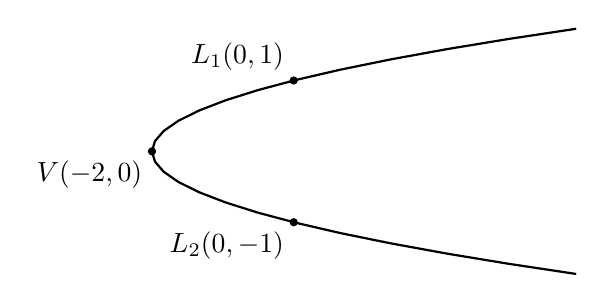
\begin{tikzpicture}[scale=0.9]
		\coordinate (V) at (-2,0);
		\coordinate (L1) at (0,1);
		\coordinate (L2) at (0,-1);
		
		\tkzInit[xmin=-4,ymin=-3,xmax=4,ymax=3]
		\tkzGrid
		\tkzAxeXY
		
		\draw[thick, domain=-1.73:1.73] plot ({2*\x*\x-2},\x);
		
		\filldraw (V) circle (0.05)
		node[below left]{$V(-2,0)$};
		\filldraw (L1) circle (0.05)
		node[above left]{$L_1(0,1)$};
		\filldraw (L2) circle (0.05)
		node[below left]{$L_2(0,-1)$};
	\end{tikzpicture}
\end{center}
Troviamo subito gli altri due vertici dell'ellisse sostituendo $x=0$ nell'equazione della parabola
\begin{equation*}
y^2=1 \rightarrow y = \pm 1 \rightarrow L(0,\pm1)
\end{equation*}
E ora possiamo trovare l'ellisse sapendo che passa attraverso $V$ e $L_1$ (bastano solo questi due
vertici in quanto è simmetrica).
\begin{equation*}
\begin{dcases}
\frac{4}{a}=1\\
\frac{1}{b}=1
\end{dcases} \rightarrow
\begin{cases}
a=4\\
b=1
\end{cases} \rightarrow \boxed{\mathscr{E}:\,\frac{x^2}{16}+y^2=1}
\end{equation*}
Prima di disegnarla, osserviamo il punto successivo: ci chiede i punti dell'ellisse che si trovano ad
una certa distanza da $V$. Abbiamo un paio di modi, uno di questi è immaginare una circonferenza di
centro $V$ che abbia raggio pari alla distanza richiesta e vedere le intersezioni con l'ellisse.

\begin{center}
	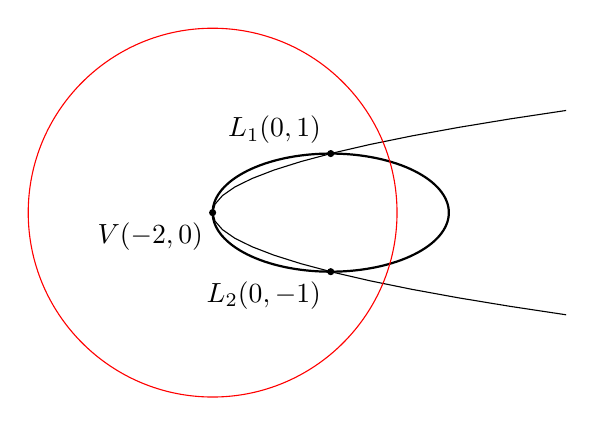
\begin{tikzpicture}[scale=0.75]
	\coordinate (V) at (-2,0);
	\coordinate (L1) at (0,1);
	\coordinate (L2) at (0,-1);
	
	\def\R{sqrt(39)/2};
	
	\tkzInit[xmin=-6,ymin=-4,xmax=4,ymax=4]
	\tkzGrid
	\tkzAxeXY
	
	\draw[domain=-1.73:1.73] plot ({2*\x*\x-2},\x);
	\draw[thick] ellipse (2 and 1);
	\draw[red] (V) circle (\R);
	
	\filldraw (V) circle (0.05)
	node[below left]{$V(-2,0)$};
	\filldraw (L1) circle (0.05)
	node[above left]{$L_1(0,1)$};
	\filldraw (L2) circle (0.05)
	node[below left]{$L_2(0,-1)$};
	\end{tikzpicture}
\end{center}

La nostra circonferenza è
\begin{equation*}
(x-x_0)^2+(y-y_0)^2=r \rightarrow \mathscr{C}:\,(x+2)^2 + y^2 = \left(\frac{\sqrt{39}}{2}\right)^2
\end{equation*}

Per trovare i punti di intersezione, mettiamo a sistema le due equazioni
\begin{align*}
&\begin{dcases}
(x+2)^2+y^2=\frac{39}{4}\\
x^2+4y^2=4
\end{dcases}\rightarrow
\begin{dcases}
y^2 = \frac{-4x^2-16x-23}{4}\\
x^2+4\cdot\frac{-4x^2-16x-23}{4}=4
\end{dcases}\rightarrow\\
&\begin{dcases}
y^2 = \frac{-4x^2-16x-23}{4}\\
\begin{dcases}
x_1 = -\frac{19}{3}\\
x_2 = 1
\end{dcases}
\end{dcases}\rightarrow
\begin{dcases}
\begin{dcases}
y_1 = \pm\frac{5\sqrt{13}\imath}{6}\\
y_2 = \pm\frac{\sqrt{3}}{2}
\end{dcases}\\
\begin{dcases}
x_1 = -\frac{19}{3}\\
x_2 = 1
\end{dcases}
\end{dcases}
\end{align*}
Da queste soluzioni, eliminiamo quelle che non appartengono ad $\mathbb{R}$ e quindi otteniamo
i punti di intersezione
\begin{equation*}
\boxed{P_1\left(1,\frac{\sqrt{3}}{2}\right)\qquad P_2\left(1,-\frac{\sqrt{3}}{2}\right)}
\end{equation*}

\subsection*{\hyperref[sec:goniometria]{Goniometria}}\label{ex:goniometria}
\paragraph{Esercizio 1}
Risolvere la seguente equazione
\begin{equation*}
(\sqrt{3}+2)\cos x + \sin x + 1 =0
\end{equation*}
\divisor

Abbiamo già la fortuna che questa equazione è già stata semplificata ed organizzata. Notiamo 
osservandola che si tratta di un'equazione goniometrica lineare. Quindi procediamo con la risoluzione
\begin{align*}
\intertext{Poniamo}
&\cos x = X\,\text{e } \sin x = Y\\
&\begin{cases}
(\sqrt{3}+2)X + Y + 1 = 0\\
X^2+Y^2 = 1
\end{cases} \rightarrow\\
&\begin{cases}
Y = -1-(\sqrt{3}+2)X\\
X^2+1+(7+4\sqrt{3})X^2+2(2+\sqrt{3})X = 1
\end{cases}\\
\intertext{Quindi otteniamo le due possibili soluzioni}
&\begin{cases}
X = 0\\ Y=--1
\end{cases}\,\text{e }
\begin{dcases}
X = -\frac{1}{2}\\ Y = \frac{\sqrt{3}}{2}
\end{dcases}
\end{align*}
I due sistemi rappresentano le intersezioni con la circonferenza quindi ora non resta che trovare 
quali angoli (o archi) intersecano la circonferenza in quelle posizione. Ed essi sono
\begin{equation*}
x = \frac{2}{3}\pi + 2k\pi \qquad x = \frac{3}{2}\pi + 2k\pi
\end{equation*}

\paragraph{Esercizio 2}
Risolvere la seguente equazione
\begin{equation*}
\sin^2x + (1-\sqrt{3})\sin x\cos x-\sqrt{3}\cos^2 x = 0
\end{equation*}
\divisor

Notiamo che l'equazione è omogenea in quanto tutti i suoi termini sono di secondo grado. Dato che \\
contiene sia il termine di secondo grado in $\sin x$ sia in $\cos x$, possiamo scegliere per cosa 
dividere. Per preferenza personale, dividiamo per $\cos^2 x$.
\begin{align*}
&\frac{\sin^2x + (1-\sqrt{3})\sin x\cos x-\sqrt{3}\cos^2 x}{\cos^2 x} = 0 \rightarrow\\
&\tan^2 x + (1-\sqrt{3})\tan x - \sqrt{3} = 0
\intertext{che risolta dà}
(\tan x)_{1/2} &= \frac{\sqrt{3}-1\pm\sqrt{1+3-2\sqrt{3}+4\sqrt{3}}}{2} =\\
&\frac{\sqrt{3}-1\pm(1-\sqrt{3})}{2} = \begin{cases}
\tan x = -1\\\tan x = \sqrt{3}
\end{cases}
\intertext{che forniscono le soluzioni}
&x = -\frac{\pi}{4}+k\pi\,\text{e } x = \frac{\pi}{3}+k\pi
\end{align*}

\paragraph{Esercizio 3}
Nel settore circolare $AOB$ di raggio $r$, centro $O$ e angolo di apertura di $\ang{60}$ è inscritto
il rettangolo $MNPQ$ avente il vertice $M$ sull'arco $\arc{AB}$, il vertice $N$ sul raggio $OB$ e il
lato $PQ$ su $OA$. Determinare la posizione del vertice $M$ in modo che l'area di detto rettangolo
valga $\dfrac{\sqrt{3}}{6}r^2$.
\divisor

Per prima cosa, facciamo il disegno
\begin{center}
	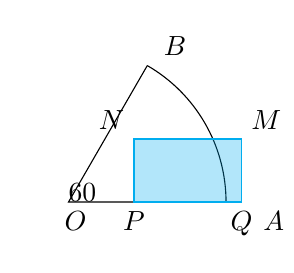
\begin{tikzpicture}[scale=2]
		\coordinate (O) at (0,0);
		\coordinate (A) at (1,0);
		\coordinate (B) at (0.5,0.866);
		\coordinate (P) at (0.24,0);
		\coordinate (Q) at (0.923,0);
		\coordinate (N) at (0.24,0.4);
		\coordinate (M) at (0.923,0.4);
		
		\draw (A) -- (O) -- (B);
		\draw (A) arc(0:60:1);
		\markangle{O}{A}{B}{0.2}{2}{$\ang{60}$}
		\filldraw[cyan, fill opacity = 0.3] (P) -- (Q) -- (M) -- (N) -- cycle;
		\node (A1) at (A) [below right]{$A$};
		\node (B1) at (B) [above]{$B$};
		\node (P1) at (P) [below]{$P$};
		\node (Q1) at (Q) [below]{$Q$};
		\node (O1) at (O) [below left]{$O$};
		\node (N1) at (N) [above left]{$N$};
		\node (M1) at (M)[above right]{$M$};
	\end{tikzpicture}
\end{center}
Da questo possiamo dire che l'area di un rettangolo qualsiasi è definita come
$\text{base}\cdot\text{altezza}$, in questo caso come $\overline{PQ}\cdot\sin(\theta)r$ ($r$ è 
inserito per avere il seno corretto qualunque sia il raggio, $\theta = \arc{AOM}$). Il problema ora 
è trovare $\overline{PQ}$.\\
Definiamo $y_M$ e $y_N$ le due ordinate dei rispettivi punti.
\begin{equation*}
y_N = \overline{ON}\sin(\ang{60}) = y_M = r\sin(\theta)
\end{equation*} 
Questo lo vediaom chiaramente dal disegno.\\
$P$ si trova al piede di $N$, quindi la sua coordinata è
\begin{equation*}
\frac{y_N}{\tan(\ang{60})} = \frac{r\sin\theta}{\tan(\ang{60})}
\end{equation*}
Perché da $y_N = \overline{ON}\sin(\ang{60})$ abbiamo isolato $\overline{ON}$ e moltiplicato per il
$\cos(\ang{60})$.\\
Infine $Q$ si trova al $\cos\theta$. Con queste informazioni, possiamo scrivere che
\begin{align*}
&\frac{\sqrt{3}}{6}r^2 = \left(r\cos\theta - \frac{r\sin\theta}{\tan(\ang{60})}\right)r\sin\theta\\
\intertext{Raccogliendo e semplificando $r$, risolvendo $\tan(\ang{60})$}
&\frac{1}{2\sqrt{3}} = \sin\theta\cos\theta -\frac{\sin^2\theta}{\sqrt{3}}\\
\intertext{Sostituiamo $\cos\theta = \sqrt{1-\sin^2\theta}$}
&\frac{1}{2\sqrt{3}} = \sin\theta\sqrt{1-\sin^2\theta}-\frac{\sin^2\theta}{\sqrt{3}}\\
\intertext{Poniamo $\sin\theta = t$}
&\frac{1}{2\sqrt{3}} = t\sqrt{1-t^2}-\frac{1}{\sqrt{3}}t^2\\
\intertext{Moltiplichiamo per $2\sqrt{3}$}
&1 = 2\sqrt{3}t\sqrt{1-t^2}-2t^2\\
\intertext{Spostiamo $t^2$}
&1+2t^2 = 2\sqrt{3}t\sqrt{1-t^2}\\
\intertext{Eleviamo al quadrato}
&1+4t^2+4t^4 = 12t^2-14t^4\\
\intertext{Semplifichiamo}
&-16t^4+8t^2-1=0\\
\intertext{Poniamo $u = t^2$}
&-16u^2-8u-1=0\\
\intertext{Risolviamo per $u$}
&u = \frac{1}{4}\\
\intertext{Torniamo a sostituire $t^2=u$}
&t = \sqrt{\frac{1}{4}} = \pm\frac{1}{2}\\
\intertext{Verifichiamo che solo $\dfrac{1}{2}$ è soluzione e torniamo a sostituire $t = \sin\theta$}
&\sin\theta = \frac{1}{2} \rightarrow \theta = \arcsin\left(\frac{1}{2}\right) = \boxed{\ang{30}}
\end{align*}

\subsection*{\hyperref[sec:logaritmi]{Logaritmi}}\label{ex:logaritmi}
\paragraph{Esercizio 1}
Risolvi
\begin{equation*}
50\left(\frac{4}{25}\right)^x-133\left(\frac{2}{5}\right)^x+20=0
\end{equation*}
\divisor

Per risolvere questo tipo di equazioni in modo semplice possiamo osservare attentamente e notare che
il primo termine tra parentesi ($\dfrac{4}{25}$) non è altro che il quadrato del secondo 
($\dfrac{2}{5}$)! Questo ci porta riscrivere l'equazione come
\begin{equation*}
50\left(\frac{2}{5}\right)^{2x}-133\left(\frac{2}{5}\right)+20=0
\end{equation*}
E ora possiamo risolvere semplicemente.
\begin{align*}
\intertext{Poniamo}
&t = \left(\frac{2}{5}\right)^x\\
\intertext{si ha quindi}
&50t^2-133t+20=0\\
&t_{1/2} = \frac{133\pm\sqrt{133-4\cdot50\cdot20}}{100} = \frac{133\pm117}{100}\\
&\begin{dcases}
t_1 = \frac{5}{2}\\
t_2 = \frac{4}{25}
\end{dcases}
\intertext{Torniamo a sostituire per $t_1$}
&\left(\frac{2}{5}\right)^x = \frac{5}{2}\rightarrow x = \log_{\frac{2}{5}}\frac{5}{2}
\intertext{Ricordando la proprietà $\log_{\frac{1}{a}} b = -\log_a b$}
&x = -\log_{\frac{5}{2}}\frac{5}{2} = \boxed{-1}
\intertext{Sostituiamo per $t_2$}
&\left(\frac{2}{5}\right)^x = \frac{4}{25}\rightarrow x = \log_{\frac{2}{5}}\frac{4}{25}
\intertext{Ricordando che $\log_a b^k = k\log_a b$}
&x = 2\log_{\frac{2}{5}}\frac{2}{5} = \boxed{2}
\end{align*}

\subsection*{\hyperref[sec:progressioni]{Progressioni}}\label{ex:progressioni}
\paragraph{Esercizio 1}
Trovare la somma dei primi $8$ termini di una progressione geometrica sapendo che il secondo termine
è $4$ e il quinto è $108$.

\divisor

Indichiamo come $a_1$ il primo termine e $q$ la ragione. Possiamo ora scrivere un sistema che ci
"matematizza" ciò che ci viene detto
\begin{align*}
&\begin{cases}
a_1q = 4\\
a_1q^4=108
\end{cases}
\intertext{da questo possiamo dividere membro a membro}
&\frac{a_1q}{a_1q^4}=q^3=\frac{108}{4}=27 \rightarrow q = 3
\intertext{Sostituendo nella prima equazione}
&a_1 = \frac{4}{3}
\intertext{E possiamo quindi trovare la somma di $8$ elementi}
&S_n = a_1\frac{1-q^n}{1-q} \rightarrow S_8 =
\frac{4}{3}\cdot\frac{1-3^8}{1-3}=\boxed{\frac{13120}{3}}
\end{align*}

\paragraph{Esercizio 2}
Una progressione aritmetica ha il primo termine $a_1=a$ e ragione $d=10$. La somma dei primi $n$ 
termini è pari a $10000$. Determinare l'espressione che fornisce $a_1$ in funzione di $n$ e calcolare
il valore di $a_{20}$.

\divisor

Ricordando la formula per la somma di una progressione
\begin{equation*}
S_n = \frac{a_1+a_n}{2}n
\end{equation*}
vediamo che per trovare $a_1$ ci manca solo $a_n$. Per trovarlo usiamo la formula per trovare
l'$n$-esimo elemento
\begin{align*}
&a_n = a_1+d(n-1) \rightarrow a_n = a+dn-d = a_n = a+10n-10
\intertext{A questo punto riscriviamo la formula della somma con tutti i dati}
&10000 = \frac{a+a+10n-10}{2}n\rightarrow 20000 = 2an+10n^2-10n
\intertext{Isoliamo $a$}
&\boxed{a = \frac{10000}{n}-5n+5}
\end{align*}

A questo punto troviamo l'elemento riapplicando la formula
\begin{equation*}
a_{20} = a_1 + d(20-1) = \frac{10000}{20}-5\cdot20+5+10\cdot(20-1) =\boxed{595} 
\end{equation*}

\subsection*{\hyperref[sec:calccomb]{Calcolo combinatorio}}\label{ex:calccomb}
\paragraph{Esercizio 1}
Determinare in quanti modi è possibile estrarre due carte da un mazzo di $52$ in modo che
\begin{itemize}
	\item le due carte estratte siano entrambe rosse
	\item una sia rossa e l'altra nera
	\item una almeno sia rossa
\end{itemize}
\divisor

Per il primo punto vediamo che ci chiedono 2 carte rosse. Un mazzo da $52$ contiene $26$ nere e 
altrettante rosse essendo un mazzo di carte francesi. Dato che l'ordine non ha importanza e che
tutti gli elementi sono distinti, le possibilità sono le combinazioni semplici. Quindi
\begin{equation*}
\boxed{\binom{26}{2}}
\end{equation*}
$26$ perché ci interessano solo le rosse, non tutto il mazzo.\\ [\baselineskip]
Il prossimo punto chiede una carta rossa e una carta nera. Immaginiamo di avere quindi due spazi. Nel
primo mettiamo una carta rossa (quindi $26$ possibilità), nel secondo una nera (sempre $26$). Quindi
le totali possibilità si ottengono semplicemente moltiplicando
\begin{equation*}
26\cdot26 = \boxed{676}
\end{equation*}
Per l'ultimo punto, dobbiamo sottrarre da tutte le possibilità quelle che non contengono una carta 
rossa. Dato che ci viene detto \emph{almeno} una rossa, possono essere anche entrambe. Quindi
\begin{equation*}
\boxed{\binom{52}{2}-\binom{26}{2}}
\end{equation*}

\paragraph{Esercizio 2}
Dimostrare
\begin{equation*}
\binom{n}{k+1} = \binom{n}{k}\frac{n-k}{k+1}
\end{equation*}
\divisor

\begin{align*}
\intertext{Partiamo sviluppando il lato sinistro}
&\binom{n}{k+1} = \frac{n!}{(k+1)!(n-k-1)!} = \frac{n!}{k!(k+1)(n-k-1)!}
\intertext{Se osserviamo attentamente notiamo che ci manca semplicemente un $n-k$ da aggiungere per
ottenere il desiderato. Quindi possiamo moltiplicare per $n-k$ e ottenere}
&\frac{n!}{k!(k+1)(n-k-1)!} = \binom{n}{k}\frac{n-k}{k+1}
\intertext{Q.E.D.}
\end{align*}

\subsection*{\hyperref[sec:prob]{Probabilità}}\label{ex:prob}
\paragraph{Esercizio 1}
Tre macchine utensili producono lo stesso tipo di pezzi. La prima ne produce $150$ al giorno con il 
$2\%$ dei pezzi difettosi, la seconda ne produce $500$ con il $5\%$ di pezzi difettosi, la terza
$50$ con nessun pezzo difettoso. Supponiamo ora di prendere un pezzo a caso della produzione di un 
dato giorno, calcolare la probabilità che
\begin{enumerate}
	\item il pezzo sia stato prodotto dalla prima macchina
	\item il pezzo sia stato prodotto dalla seconda macchina
	\item il pezzo sia stato prodotto dalla terza macchina
	\item il pezzo sia difettoso
\end{enumerate}
Supponendo che il pezzo sia difettoso, calcolare la probabilità che
\begin{enumerate}
	\item sia stato prodotto dalla prima macchina
	\item sia stato prodotto dalla seconda macchina
	\item sia stato prodotto dalla terza macchina
\end{enumerate}
\divisor

Una cosa che ritorna estremamente utile nella risoluzione dei problemi di probabilità è il grafico ad
albero per mostrare tutte le possibilità. Come questo

\begin{center}
	\begin{tikzpicture}
		\tikzset{level 1/.style={level distance = 40pt}}
		\tikzset{level 2/.style={level distance = 40pt}}
		\Tree [.\node (Produzione) {Produzione};
			[.\node (Prima) {Prima};
				[.\node (Buono1) {Buono};
					$\dfrac{147}{600}$
				]
				[.\node (Difettoso1) {Difettoso};
					$\dfrac{3}{600}$
				]
			]
			[.\node (Seconda) {Seconda};
				[.\node (Buono2) {Buono};
					$\dfrac{380}{600}$
				]
				[.\node (Difettoso2) {Difettoso};
					$\dfrac{20}{600}$
				]
			]
			[.\node (Terza) {Terza};
				[.\node (Buono3) {Buono};
					$\dfrac{50}{600}$
				]
				[.\node (Difettoso3) {Difettoso};
					$0$
				]
			]
		]
		\node[above] at ($(Produzione) !.5! (Prima)$) {$\dfrac{150}{600}$};
		\node[left] at ($(Produzione) !.6! (Seconda)$) {$\dfrac{400}{600}$};
		\node[above] at ($(Produzione) !.5! (Terza)$) {$\dfrac{50}{600}$};
		\node[left] at ($(Prima) !.5! (Buono1)$) {$\dfrac{2}{100}$};
		\node[right] at ($(Prima) !.5! (Difettoso1)$) {$\dfrac{98}{100}$};
		\node[left] at ($(Seconda) !.5! (Buono2)$) {$\dfrac{5}{100}$};
		\node[right] at ($(Seconda) !.5! (Difettoso2)$) {$\dfrac{95}{100}$};
		\node[left] at ($(Terza) !.5! (Buono3)$) {$0$};
		\node[right] at ($(Terza) !.5! (Difettoso3)$) {$\dfrac{100}{100}$};
	\end{tikzpicture}
\end{center} 

I risultati che si vedono sono semplicemente ricavati dal prodotto delle due probabilità
secondo la formula $p\left(\mathbb{E}_1\cap\mathbb{E}_2\right) = p(\mathbb{E}_1)\cdot p(\mathbb{E}_2)$
.\\[\baselineskip]
In totale vi sono $23$ pezzi difettosi in un giorno (infatti se andiamo ad osservare i numeratori e 
sommiamo i difettosi vediamo $3+20+0 = 23$). Quindi la probabilità che un pezzo sia difettoso è
\begin{equation*}
p(\text{Difettoso}) = \frac{23}{600} \approx \boxed{3.8\%}
\end{equation*}

Allora, la probabilita che sia difettoso e dalla prima macchina è
\begin{equation*}
p\left(\text{Prima}\mid\text{Difettoso}\right) = \frac{\frac{3}{600}}{\frac{23}{600}} 
\approx\boxed{13\%}
\end{equation*}
e dalla seconda
\begin{equation*}
p\left(\text{Seconda}\mid\text{Difettoso}\right) = \frac{\frac{20}{600}}{\frac{23}{600}} 
\approx\boxed{8.7\%}
\end{equation*}

\subsection*{\hyperref[sec:aff]{Affinità}}\label{ex:aff}
\paragraph{Esercizio 1}
Data l'affinità
\begin{equation*}
T:\,\begin{cases}
x'=2x+y-1\\y'=x-y-2
\end{cases}
\end{equation*}
determinare
\begin{enumerate}
	\item il punto unito $U$
	\item i trasformati $O'$, $A'$ e $B'$ dei punti $O(0,0)$, $A(2,-1)$, $B(-3,4)$ e l'area del 
	triangolo $A'O'B'$
	\item la trasformazione inversa $T^{-1}$
	\item le trasformate delle curve
	\begin{equation*}
	y=3x+4\qquad x-y+5=0\qquad y=x^2
	\end{equation*}
\end{enumerate}
\divisor

Trovare il punto unito di $T$ è semplice, basta solo porre $x'=x$ e $y'=y$.
\begin{align*}
&\begin{cases}
x=2x+y-1\\
y=x-y-2
\end{cases}
\begin{cases}
y = -x+1\\
-x+1=x+x-4
\end{cases}
\begin{cases}
y=\frac{1}{3}\\
x=\frac{4}{3}
\end{cases}\rightarrow \\&U\left(\frac{1}{3},\frac{4}{3}\right)
\end{align*}

Trovare i trasformati è estremamente semplice: basta sostituire i valori di $x$ e $y$ dei punti
all'interno dell'affinità
\begin{equation*}
\boxed{
O':\,\begin{cases}
x'=-1\\y'=-2
\end{cases}
A':\,\begin{cases}
x'=4-2=2\\
y'=2+1-2=1
\end{cases}
B':\,\begin{cases}
x'=-3\\
y'=-9
\end{cases}
}	
\end{equation*}

L'area del triangolo è facilmente trovabile usando la matrice

\begin{equation*}
\mathscr{A}(ABC) = \frac{1}{2}\left\lvert 
\begin{matrix}[1]
x_1 & y_1 & 1\\
x_2 & y_2 & 1\\
x_3 & y_3 & 1
\end{matrix}\right\rvert
\end{equation*}
e risolvendola con Sarrus. Quindi inserendo i valori e risolvendo otteniamo
\begin{align*}
&\mathscr{A}(A'O'B') = \frac{1}{2}\left\lvert 
-1+(-18)+6-(-3+9-4)\right\rvert = \\&\frac{1}{2}\left\lvert 
-1-18+6+3-9+4\right\rvert = \\&\frac{1}{2}\left\lvert-15\right\rvert = \boxed{\frac{15}{2}}
\end{align*}

Trovare la trasformazione inversa richiede solo di risolvere il sistema in $x$ e $y$.
\begin{align*}
&\begin{cases}
2x+y=x'+1\\
x-y=y'+2
\end{cases}
\begin{cases}
2y'+4+3y'=x'+1\\
x='+2+y
\end{cases}\\
&\boxed{\begin{dcases}
y = \frac{x'}{3}+\frac{2}{3}y'-1\\
x = \frac{x'}{3}+\frac{y'}{3}+1
\end{dcases}}
\end{align*}


Trovare le trasformate di un'equazione è relativamente semplice. Piuttosto tedioso per alcune formule
ma non complicato. Quello che si fa è applicare la trasformazione inversa alla nostra equazione.
Questo perché immaginiamo che ciò che abbiamo sia un risultato e noi dobbiamo trovare l'equazione
che ha portato a quella data. Quindi torniamo indietro e dunque usiamo l'inversa.
\begin{align*}
&y=3x+4 \rightarrow\\
&\frac{x'}{3}-\frac{2}{3}y'-1=3\left(\frac{x'}{3}+\frac{y'}{3}+1\right)+4 \rightarrow\\
&\frac{x'}{3}-\frac{2}{3}y'-1=x'+y'+7\rightarrow\\\Aboxed{&2x'+5y'+24=0}
\end{align*}
\begin{align*}
&x-y+5=0\rightarrow\\
&\cancel{\frac{x'}{3}}+\frac{y'}{3}+1-\cancel{\frac{x'}{3}}+\frac{2}{3}y'+1+5 \rightarrow
\boxed{y'+5=0}
\end{align*}
\begin{align*}
&y=x^2\rightarrow\\
&0=-\frac{x'}{3}+\frac{2}{3}y'+1+\frac{x'}{9}+\frac{2}{9}xy+\frac{2}{9}x+\frac{y^2}{9}+\frac{2}{9}y+1
\\ &\boxed{x^{'2}+2x'y'+y^{'2}+3x'+12y'+18=0}
\end{align*}

\paragraph{Esercizio 2}
Considera nel piano $xOy$ la famiglia di curve di equazione
\begin{equation*}
y=\frac{mx-8}{x-2m}
\end{equation*}
determinare:
\begin{enumerate}
	\item per quali valori di $m$ l'equazione rappresenta un'iperbole equilatera traslata e il luogo
	di simmetria delle iperboli della famiglia \label{enum:ex:aff:2:1}
	\item le iperboli $\Phi_1$ e $\Phi_2$ della famiglia che sono tangenti, nel loro punto di ascissa
	nulla, alla retta con coefficiente angolare $\dfrac{1}{2}$. Sia $\Phi_1$ quella relativa al valore
	$m>0$ \label{enum:ex:aff:2:2}
	\item il luogo $\gamma$ dei centri delle circonferenze passanti per $O$ e tangenti al luogo
	di simmetria delle iperboli \label{enum:ex:aff:2:3}
	\item detta $\theta'$ la curva corrispondente di $\theta$ nella trasformazione
	\label{enum:ex:aff:2:4}
	\begin{equation*}
	\begin{dcases}
	x = \frac{\sqrt{2}}{2}x'-\frac{\sqrt{2}}{2}y'\\
	y = \frac{\sqrt{2}}{2}x'+\frac{\sqrt{2}}{2}y'
	\end{dcases}
	\end{equation*}
	determinare il punto $P$ di $\theta'$ nel primo quadrante in corrispondenza del quale è \\
	\textbf{massima} l'area del quadrilatero $OVPM$ essendo $V$ il punto di $\theta'$ di ordinata
	nulla e $M$ il punto di intersezione di $\theta'$ con i semiasse negativo delle ordinate.
	Sia $\theta$ la circonferenza con raggio pari a $1$ che si trova nella parte positiva di $y$.
\end{enumerate}
\divisor

Per il \hyperref[enum:ex:aff:2:1]{\textbf{punto uno}} dobbiamo vedere in che caso l'equazione non
descrive più un'iperbole. Per fare questo proviamo a semplificare e vediamo che dividendo
\begin{equation*}
\frac{mx}{x} \quad \text{e} \quad \frac{8}{2m}
\end{equation*}
otteniamo
\begin{equation*}
m = \frac{8}{2m} \rightarrow m^2 = 4 \rightarrow \boxed{m=\pm2}
\end{equation*}
Quindi i valori che noi dobbiamo esculdere sono $m\neq\pm2$ in quanto annullano l'equazione che
diventerebbe una retta passante per $y=\pm2$.\\
Il luogo dei centri di simmetria è quella retta su cui giaciono tutti i centri. Un centro è il punto
\begin{equation*}
C\left(-\frac{d}{c},\frac{a}{c}\right)
\end{equation*}
ed inserendo i nostri valori otteniamo
\begin{equation*}
C(2m,m)
\end{equation*}
quindi il luogo è dato dall'equazione $\boxed{y=\dfrac{x}{2}}$. Dobbiamo però escludere i punti
\begin{equation*}
(4,2)\qquad(-4,-2)
\end{equation*}
in quanto abbiamo escluso $m=\pm2$.\\[\baselineskip]

Per il \hyperref[enum:ex:aff:2:2]{punto due} possiamo trovare i punti che distano $0$ dal fascio di
rette $y=\dfrac{1}{2}x+q$ e che appartengono alla nostra famiglia di iperboli che al tempo stesso
hanno $x=0$ ma non otterremmo nulla di significativo.\\
Perché? Guardiamo un attimo il disegno
\begin{center}
  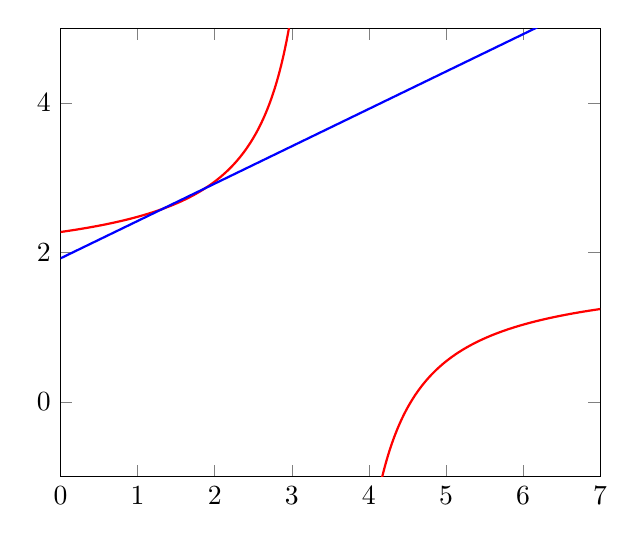
\begin{tikzpicture}
    \begin{axis}[domain=0:7, xmin=0,ymin=-1,xmax=7,ymax=5]
      \addplot[restrict y to domain=-2:6, samples=500, red, thick] {(1.76*x-8)/(x-2*1.76)};
      \addplot[blue, thick] {x/2+1.92};
    \end{axis}
   \end{tikzpicture}
\end{center}
Notiamo che per due valori di $q$ e $m$ scelti appositamente il più vicino punto di intersezione tra 
la retta e l'iperbole ha come ascissa un valore leggermente inferiore a $2$. Andando a disegnare altre
iperboli e altre rette modificando i due parametri si andrà a notare che è impossibile che la retta
$y=\dfrac{x}{2}+q$ per qualunque $q$ sia tangente all'iperbole $\Phi$ in modo che $x=0$.\\[\baselineskip]

Per il \hyperref[enum:ex:aff:2:3]{punto tre} abbiamo un problema interessante. Abbiamo una 
circonferenza che passa per $O(0,0)$ e il cui centro abbia distanza dalla retta pari al raggio.
Scriviamo quindi il sistema
\begin{align*}
&\begin{dcases}
c = 0\\
\frac{\left\lvert -\frac{a}{4}+\frac{b}{2}+c\right\rvert}{\sqrt{a^2+b^2}}=
\sqrt{\frac{a^2}{4}+\frac{b^2}{4}-c}
\end{dcases}\rightarrow
\frac{\left\rvert a-2b\right\rvert}{2\sqrt{5}}=\sqrt{\frac{a^2}{4}+\frac{b^2}{4}}
\intertext{Semplifichiamo e otteniamo}
&b = -2a
\end{align*}
Cosa ci dice questo? Proviamo a inserire le informazioni all'interno della coordinata del centro
\begin{equation*}
C\left(-\frac{a}{2},-\frac{b}{2}\right)\rightarrow C\left(-\frac{a}{2},a\right)
\end{equation*}
Da questo vediamo che $y=-2x$. Quindi il nostro luogo dei centri è
\begin{equation*}
\boxed{\gamma:\,y = -2x}
\end{equation*}

Avremmo potuto farlo in un altro modo? Con un po' di ragionamento, sì, senza dubbio. Sappiamo che
le circonferenze devono passare per $O(0,0)$ e essere tangenti a $y=\dfrac{x}{2}$. Però anche questa
retta passa per $O(0,0)$ in quanto ha $q=0$. Quindi il punto di tangenza è esattamente il centro degli
assi. Se sappiamo questo e sappiamo che le circonferenze devono essere tangenti, significa che 
sappiamo il raggio è perpendicolare alla retta. Quindi la retta passante per il centro e 
perpendicolare a $y=\dfrac{x}{2}$ è proprio $y=-2x$.\\\

Per il \hyperref[enum:ex:aff:2:4]{punto quattro} troviamo la circonferenza che ha il centro su quella
retta e che abbia il raggio pari a $1$.
\begin{align*}
\intertext{L'equazione della generica circonferenza è }
&x^2+y^2+ax-2ay=0
\intertext{perché avendo visto prima la soluzione dell'equazione del luogo geometrico sappiamo che
$b=-2a$. Scriviamo tutto in funzione di $a$ per comodità.
Con questo chiarito, troviamo il valore di $a$ sapendo che il raggio è pari a $1$}
&\sqrt{\frac{a^2}{4}+a^2} = 1 \rightarrow \frac{4}{5}a^2=1 \rightarrow a=\pm\frac{2\sqrt{5}}{5}
\intertext{Per scegliere quale dei due è accettabile, disegnamoli}
\end{align*}

\begin{center}
	\begin{tikzpicture}[scale=2]
		\coordinate (C) at (1/4.46,-1/2.23);
		\coordinate (C1) at (-1/4.46,1/2.23);
		\tkzInit[xmin=-1,ymin=-1,xmax=1,ymax=1]
		\tkzGrid
		\tkzAxeXY
		
		\draw[red, thick] (C) circle (1/2);
		\draw[blue, thick] (C1) circle (1/2);
		\filldraw[red] (C) circle (0.025);
		\filldraw[blue] (C1) circle (0.025);
		\node[red, below] at (C) {$a=\dfrac{2\sqrt{5}}{5}$};
		\node[blue, above] at (C1) {$a=-\dfrac{2\sqrt{5}}{5}$};
	\end{tikzpicture}
\end{center}
Quindi tra queste due quella da scegliere è quella con $a < 0$. Scriviamola
\begin{equation*}
\theta:\,x^2+y^2-\frac{2\sqrt{5}}{5}x+\frac{4\sqrt{5}}{5}y=0
\end{equation*}
La trasformazione che dobbiamo applicare è
\begin{equation*}
\begin{dcases}
x = \frac{\sqrt{2}}{2}x'-\frac{\sqrt{2}}{2}y'\\
y = \frac{\sqrt{2}}{2}x'+\frac{\sqrt{2}}{2}y'
\end{dcases}
\end{equation*}
che osservandola rappresenta una rotazione di $\alpha=\ang{45}$. Come mai? Beh, abbiamo la matrice dei
coefficienti che è
\begin{equation*}
\begin{bmatrix}[2.5]
\dfrac{\sqrt{2}}{2} & -\dfrac{\sqrt{2}}{2}\\
\dfrac{\sqrt{2}}{2} & \dfrac{\sqrt{2}}{2}
\end{bmatrix}
\end{equation*}
che messa accanto a quella della rotazione
\begin{equation*}
\begin{bmatrix}[1]
\cos\theta & -\sin\theta\\
\sin\theta & \cos\theta
\end{bmatrix}
\end{equation*}
risultano estremamente simili con $\theta = \dfrac{\pi}{4}$. Tanto simili da coincidere. Quindi 
sappiamo che abbiamo una rotazione di $\ang{45}$. Applichiamo la trasformazione inversa alla nostra
equazione e otteniamo
\begin{align*}
&\left(\frac{\sqrt{2}}{2}x'-\frac{\sqrt{2}}{2}y'\right)^2+
\left(\frac{\sqrt{2}}{2}x'+\frac{\sqrt{2}}{2}y'\right)^2+\\
&-\frac{2\sqrt{5}}{5}\left(\frac{\sqrt{2}}{2}x'-\frac{\sqrt{2}}{2}y'\right)+
\frac{4\sqrt{5}}{5}\left(\frac{\sqrt{2}}{2}x'+\frac{\sqrt{2}}{2}y'\right) = 0
\intertext{Che semplificata tramite calcoli che non riporto perché eccessivamente lunghi}
&\boxed{\theta':\,x'^2+y^2+\sqrt{\frac{2}{5}}x+3\sqrt{\frac{2}{5}}y = 0}
\end{align*}
Che disegnata è
\begin{center}
	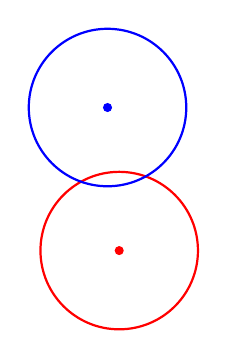
\begin{tikzpicture}[scale=2]
	\coordinate (C) at (-0.15,-0.46);
	\coordinate (C1) at (-1/4.46,1/2.23);
	
	\tkzInit[xmin=-1,ymin=-1,xmax=1,ymax=1]
	\tkzGrid
	\tkzAxeXY
	
	\draw[red, thick] (C) circle (1/2);
	\draw[blue, thick] (C1) circle (1/2);
	\filldraw[red] (C) circle (0.025);
	\filldraw[blue] (C1) circle (0.025);
	\end{tikzpicture}
\end{center}

Disegnamo ora i punti che ci vengono forniti
\begin{center}
	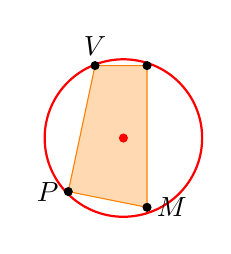
\begin{tikzpicture}[scale=2]
	\coordinate (C) at (-0.15,-0.46);
	\coordinate (V) at (-0.33,0);
	\coordinate (M) at (0,-0.9);
	\coordinate (O) at (0,0);
	\coordinate (P) at (-0.5,-0.8);
	
	\tkzInit[xmin=-1,ymin=-1,xmax=1,ymax=0.5]
	\tkzGrid
	\tkzAxeXY
	
	\draw[red, thick] (C) circle (1/2);
	\node[above] at (V) {$V$};
	\node[right] at (M) {$M$};
	\node[left] at (P) {$P$};
	\filldraw[orange, fill opacity = 0.3] (M) -- (P) -- (V) -- (O) -- cycle;
	\filldraw[red] (C) circle (0.025);
	\filldraw (V) circle (0.025);
	\filldraw (M) circle (0.025);
	\filldraw (O) circle (0.025);
	\filldraw (P) circle (0.025);
	\end{tikzpicture}
\end{center}
dove $P$ è un punto variabile. Per calcolare l'area massima di questo quadrilatero dobbiamo trovare
dove deve essere $P$ perché sia massima. Ovviamente deve appartenere alla circonferenza, quindi
deve essere il più lontano possibile da $V$ e $M$. Quindi il punto più distante è quello in cui
la retta passante tra lui e il centro della circonferenza è perpendicolare alla retta passante
tra i due punti. Disegnamo per far capire.

\begin{center}
	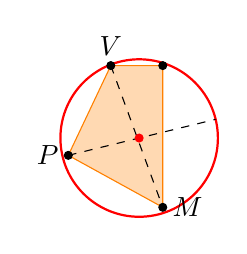
\begin{tikzpicture}[scale=2]
	\coordinate (C) at (-0.15,-0.46);
	\coordinate (V) at (-0.33,0);
	\coordinate (M) at (0,-0.9);
	\coordinate (O) at (0,0);
	\coordinate (P) at (-0.6,-0.57);
	
	\tkzInit[xmin=-1,ymin=-1,xmax=1,ymax=0.5]
	\tkzGrid
	\tkzAxeXY
	
	\draw[red, thick] (C) circle (1/2);
	\node[above] at (V) {$V$};
	\node[right] at (M) {$M$};
	\node[left] at (P) {$P$};
	
	\filldraw[orange, fill opacity = 0.3] (M) -- (P) -- (V) -- (O) -- cycle;
	
	\draw[dashed, shorten >=-1cm] (P) -- (C);
	\draw[dashed] (V) -- (M);
	
	\filldraw[red] (C) circle (0.025);
	\filldraw (V) circle (0.025);
	\filldraw (M) circle (0.025);
	\filldraw (O) circle (0.025);
	\filldraw (P) circle (0.025);
	\end{tikzpicture}
\end{center}
L'area del quadrilatero è sempre ricavabile con la matrice
\begin{equation*}
\begin{vmatrix}[1]
x_1 & y_1 & 1\\
x_2 & y_2 & 1\\
x_3 & y_3 & 1\\
x_4 & y_4 & 1
\end{vmatrix}
\end{equation*}
usando la formula di Gauss. Prima troviamo i punti
\begin{equation*}
V:\, x^2+\sqrt{\frac{2}{5}}=0 \rightarrow x = -\sqrt{\frac{2}{5}} \rightarrow 
V\left(-\sqrt{\frac{2}{5}},0\right)
\end{equation*}
\begin{equation*}
M:\,y^2+3\sqrt{\frac{2}{5}}=0 \rightarrow y = -3\sqrt{\frac{2}{5}} \rightarrow 
M\left(0,-3\sqrt{\frac{2}{5}}\right)
\end{equation*}
La retta passante tra i due punti risulta essere
\begin{equation*}
r_{VM}:\,y=-3x-3\sqrt{\frac{2}{5}}
\end{equation*}
La tangente per $P$ invece
\begin{equation*}
t_{PC}:\,y=\frac{x}{3}-\frac{4}{3}\sqrt{\frac{2}{5}}
\end{equation*}
Il punto $P$ si trova facendo l'intersezione tra la tangente e la circonferenza. Si trova quindi
\begin{equation*}
P\left(-2\sqrt{\frac{2}{5}},\frac{1}{15}(5x-4\sqrt{10})\right)
\end{equation*}
Quindi l'area massima si trova risolvendo il determinante di
\begin{equation*}
\begin{bmatrix}[2.5]
0&0&1\\
-\sqrt{\dfrac{2}{5}}&0&1\\
0&-3\sqrt{\dfrac{2}{5}}&1\\
-2\sqrt{\dfrac{2}{5}}&\dfrac{1}{15}(5x-4\sqrt{10}&1
\end{bmatrix}
\end{equation*}
che risulta essere
\begin{equation*}
\frac{1}{2}\left\lvert-\sqrt{\frac{2}{5}}\cdot\left(-3\sqrt{\frac{2}{5}}\right) -
\left(-2\sqrt{\frac{2}{5}}\cdot\left(-3\sqrt{\frac{2}{5}}\right)\right)\right\rvert
\end{equation*}
che semplificato risulta in
\begin{equation*}
\boxed{\mathscr{A}(VOMP) = \frac{3}{5}}
\end{equation*}

\subsection*{\hyperref[sec:complex]{Numeri Complessi}}\label{ex:complex}
\paragraph{Esercizio 1}
Calcolare le radici quarte di $z=2+i2\sqrt{3}$
\divisor

Calcoliamo $\rho$ e $\theta$
\begin{align*}
&\rho = \sqrt{4+12} = \sqrt{16} = 4 \quad \theta = \frac{\pi}{3}
\intertext{Quindi si ha}
&z = 4\left(\cos\frac{\pi}{3}+i\sin\frac{\pi}{3}\right)
\intertext{da cui}
&w=\sqrt[4]{z} = 
\sqrt[4]{4}\left(\cos\frac{\frac{\pi}{3}+2k\pi}{4}+i\sin\frac{\frac{\pi}{3}+2k\pi}{4}\right) =\\ 
&\sqrt{2}\left(\cos\frac{\frac{\pi}{3}+2k\pi}{4}+i\sin\frac{\frac{\pi}{3}+2k\pi}{4}\right)
\end{align*}
Le radici quarte si ottengono sostituendo a $k$ i valori in ${0,1,2,3}$. Quindi otteniamo
\begin{align*}
\Aboxed{w_1 &= \sqrt{2}\left(\cos\frac{\pi}{12}+i\sin\frac{\pi}{12}\right)}\\
w_2 &= \sqrt{2}\left(\cos\frac{\frac{\pi}{3}+2\pi}{4}+i\sin\frac{\frac{\pi}{3}+2\pi}{4}\right) = \\
\Aboxed{&\sqrt{2}\left(\cos\frac{7}{12}\pi+i\sin\frac{7}{12}\pi\right)}\\
w_3 &= \sqrt{2}\left(\cos\frac{\frac{\pi}{3}+4\pi}{4}+i\sin\frac{\frac{\pi}{3}+4\pi}{4}\right) =\\ 
\Aboxed{&\sqrt{2}\left(\cos\frac{13}{12}\pi+i\sin\frac{13}{12}\pi\right)}\\
w_4 &= \sqrt{2}\left(\cos\frac{\frac{\pi}{3}+6\pi}{4}+i\sin\frac{\frac{\pi}{3}+6\pi}{4}\right) = \\
\Aboxed{&\sqrt{2}\left(\cos\frac{19}{12}\pi+i\sin\frac{19}{12}\pi\right)}
\end{align*}

\paragraph{Esercizio 2}
Risolvere nel campo complesso
\begin{equation*}
z^2+(1-4i)z-3-3i = 0
\end{equation*}
\divisor

Applichiamo la formula risolutiva delle equazioni di secondo grado che solitamente si usa per i reali
\begin{equation*}
z_{1/2} = \frac{1-4i+\sqrt{(1-4i)^2+12+12i}}{2} = \frac{1-4i+\sqrt{-3+4i}}{2}
\end{equation*}
avendo $\sqrt{-3+4i}$ ad indicare le radici del numero complesso $-3+4i$.\\
Per determinarle poniamo
\begin{align*}
&\sqrt{-3+4i}=a+ib
\intertext{con $a,b\in\mathbb{R}$. Eleviamo al quadrato}
&-3+4i=a^2-b^2+2iab
\intertext{e imponiamo che le due parti reali e immaginarie siano uguali}
&\begin{cases}
a^2-b^2=-3\\ab=2
\end{cases}
\intertext{Ricavando $b=\frac{2}{a}$ dalla seconda equazione e sostituendolo nella prima otteniamo
un'equazione biquadratica}
&a^4+3a^2-4=0\rightarrow a^2=-8\;\text{Non accettabile e }\; x^2=1 
\intertext{da cui}
&x_1=-1\quad\text{e}\quad x_2=1
\intertext{Ricavando i corrispondendi valori di $b$ otteniamo le radici cercate}
&1-2i\quad\text{e}\quad1+2i
\intertext{Sostituendo quei valori nella prima formula}
&z_1=\frac{1-4i+1+2i}{2}=1-i\quad\text{e}\quad z_2=\frac{1-4i-1-2i}{2}=-3i
\intertext{Di conseguenza l'equazione ammette due soluzioni}
\Aboxed{&z_1=1-i\quad\text{e}\quad z_2=-3i}
\end{align*}

\subsection*{\hyperref[sec:insiemi]{Insiemi numerici}}\label{ex:insiemi}
\paragraph{Esercizio 1}
Determinare l'estremo inferiore, superiore, gli eventuali punti di accumulazione del seguente insieme
numerico
\begin{equation*}
A=\left\{x_k\in\mathbb{R}\mid x_k=\frac{1}{1-2^{-k}},\forall k\in\mathbb{N}_0\right\}
\end{equation*}
\divisor

Come vedere se ha estremi? Beh, possiamo ad esempio provare a vedere il grafico di tale funzione
\begin{center}
  \begin{tikzpicture}
    \begin{axis}[domain=-3:3, xmin=-3,ymin=-3,xmax=3,ymax=3]
      \addplot[restrict y to domain=-4:4, red, thick, samples=500] {1/(1-2^(-x))};
    \end{axis}
  \end{tikzpicture}
\end{center}
Da questo vediamo (e anche dalla formula) che descrive un'iperbole equilatera. Essendo l'iperbole una
curva che può continuare all'infinito e $k\in\mathbb{N}_0$ quindi ci sono infiniti elementi che 
proseguono in entrambi gli assi. Quindi non ci sono estremi né superiori né inferiori. O per scriverlo
in simboli
\begin{equation*}
{]{-\infty},{\infty}[}
\end{equation*}
I punti di accumulazione sono relativamente facili da trovare dal grafico. Dobbiamo trovare un punto
i cui intorni, qualunque essi siano, contengono almeno un elemento dell'insieme. Osservando il disegno
vediamo che $0$ è un punto di accumulazione in quanto sia da destra che da sinistra, diminuendo sempre
più la distanza, c'è sempre un elmento dell'insieme.

\paragraph{Esercizio 2}
Dato l'insieme di numeri reali $A=\{x\in\mathbb{R}: x= \arctan n, n\in\mathbb{N}\}$, quale delle
seguenti affermazioni è vera?
\begin{enumerate}
	\item È limitato, ma non ammette massimo
	\item È limitato e ammette sia massimo che minimo
	\item Non ha punti di accumulazione
	\item Tutte le precedenti sono false
\end{enumerate}
\divisor

Come prima cosa, facciamo il grafico.
\begin{center}
	\begin{tikzpicture}
	\tkzInit[xmin=-2,ymin=-2,xmax=2,ymax=2]
	\tkzGrid
	\tkzAxeXY
	\draw[red, thick, domain=-2:2, samples=500] plot({\x}, {rad(atan(\x))});
	\end{tikzpicture}
\end{center}
Come sappiamo, l'arcotangente tenderà ad avvicinarsi a $\pm\frac{\pi}{2}$ senza però effettivamente
raggiungerlo. Quindi non ammette né un massimo e tantomeno un minimo in quanto per qualunque valore
di $x$ ci sarà sempre un elemento corrispondente dell'insieme. Di conseguenza \textbf{sia il punto 1 
e il punto 2 falso}.\\
Punti di accomulazione ci sono? Guardiamo nuovamente il grafico. Quale punto permette di essere
sicuri che sia da sinitra che da destra ci siano intorni sempre più vicini che contengono un punto
dell'insieme. Vediamo che $0$ è un punto di questi (l'unico fra l'altro). Perché $0$ e non altro?
Prendiamo un altro punto e vediamo che per quanto ci allontaniamo o sforziamo, non garantisce che 
per	ogni punto ce ne sia uno relativo in $A$.

\subsection*{\hyperref[sec:limiti]{Limiti}}\label{ex:limiti}
\paragraph{Esercizio 1}
Verificare che
\begin{equation*}
\lim\limits_{x\to3}\frac{x^2-5x+6}{x^2-9}=\frac{1}{6}
\end{equation*}
\divisor

Consideriamo la disequazione
\begin{align*}
&\left\lvert\frac{x^2-5x+6}{x^2-9}-\frac{1}{6}<\varepsilon\right\rvert
\intertext{che per $x\neq3$ si riduce in}
&\left\lvert\frac{5x-15}{6(x+3)}\right\rvert<\varepsilon
\intertext{Da questa successivamente si ottiene}
&\begin{dcases}
\frac{5x-15}{6(x+3)}<\varepsilon\\\frac{5x-15}{6(x+3)}>-\varepsilon
\end{dcases}\rightarrow\\
&\begin{dcases}
\frac{(5-6\varepsilon)x-15-18\varepsilon}{x+3}<0\\
\frac{(5-6\varepsilon)x-15+18\varepsilon}{x+3}>0
\end{dcases}
\intertext{Risolvendo per $0<\varepsilon<\frac{5}{6}$ si ha}
&\begin{dcases}
-3<x<3\frac{5+6\varepsilon}{5-6\varepsilon}\\
x<-3;\,x>3\frac{5-6\varepsilon}{5+6\varepsilon}
\end{dcases}
\intertext{Che quindi diventa}
&
x\in{\left]3\frac{5-6\varepsilon}{5+6\varepsilon},3\frac{5+6\varepsilon}{5-6\varepsilon}\right[}-\{3\}
\end{align*}
Questo intervallo costituisce a tutti gli effetti un intorno di $3$, escluso $3$ stesso. Quindi il
limite è verificato. (Per verificare sia un intorno, si sotituiscano a $\varepsilon$ valori sempre
più vicini a $0$ (ad esempio $0.1$, $0.01$, \ldots) e si verifichi che si avvicinano sempre più ad
un valore.\\
La rappresentazione grafica di questo sistema è
\begin{center}
	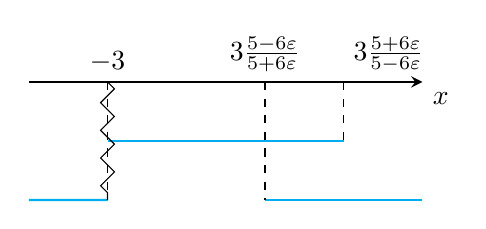
\begin{tikzpicture}[yscale=0.75]
		\coordinate (A) at (1,0);
		\coordinate (B) at (3,0);
		\coordinate (C) at (4,0);
		
		\coordinate (A1) at (1,-2);
		\coordinate (A2) at (1,-1);
		\coordinate (B1) at (3,-2);
		\coordinate (C1) at (4,-1);
		
		\draw[thick, -stealth] (0,0) -- (5,0)
			node[pos=1,below right]{$x$};
		\draw[thick, cyan] (A1) -- (0,-2);
		\draw[thick, cyan] (A2) -- (C1);
		\draw[thick, cyan] (B1) -- ++(2,0);
		\draw[dashed] (A) -- (A1);
		\draw[dashed] (B) -- (B1);
		\draw[dashed] (C) -- (C1);
		
		\draw[decorate, decoration={zigzag}] (A) -- (A1);
		
		\node[above] at (A){$-3$};
		\node[above] at (B){$3\frac{5-6\varepsilon}{5+6\varepsilon}$};
		\node[above right] at (C){$3\frac{5+6\varepsilon}{5-6\varepsilon}$};
	\end{tikzpicture}
\end{center}

\paragraph{Esercizio 2}
Verificare che
\begin{equation*}
\lim\limits_{x\to0}\ln\abs{x}=-\infty
\end{equation*}
\divisor

Consideriamo per $x\neq0$ la disequazione
\begin{equation*}
\ln\abs{x}<M
\end{equation*}
Se essa risulterà soddisfatta in un intorno di $x_0=0$ per $M<0$, lo sarà certamente per $M\geq0$.\\
Sia dunque $M<0$; si ha
\begin{equation*}
\abs{x}<e^M\quad\text{cioè}\quad-e^M<x<e^M
\end{equation*}
Pertanto il limite risulta verificato perché le soluzioni costituiscono un intorno privato dello $0$.
L'asse $y$ è asintoto verticale in questo caso.

\paragraph{Esercizio 3}
Determinare il limite di
\begin{equation*}
f(x)=\frac{2}{1-x^3}
\end{equation*}
\divisor

La funzione è definita in $\mathscr{D}_f=\mathbb{R}\setminus\{1\}$. Studiamo il segno per trovare
i limiti sinistri e destri di $x_0=1$ (in quanto è escluso dal dominio).
\begin{equation*}
1-x^3>0\rightarrow x^3<1\rightarrow x<1
\end{equation*}
Quindi quando $x<1$ è positiva, negativa altrimenti.\\
Poiché $\lim\limits_{x\to1}(1-x^3)=0$ si ha
\begin{equation*}
\boxed{\lim\limits_{x\to1^+}\frac{2}{1+x^3}=-\infty}\quad\text{e}\quad
\boxed{\lim\limits_{x\to1^-}\frac{2}{1-x^3}=+\infty}
\end{equation*}

\paragraph{Esercizio 4}
Si deduca
\begin{equation*}
\lim\limits_{x\to+\infty}\arctan\ln x
\end{equation*}
\divisor

Deducendo il limite e spezzandolo parte per parte
\begin{align*}
\lim\limits_{x\to+\infty}\ln x \to +\infty
\intertext{Questo lo si scopre anche dal grafico se non ce lo si ricorda}
\lim\limits_{x\to+\infty}\arctan+\infty\to\frac{\pi}{2}
\end{align*}
Questo lo si capisce dal grafico
\begin{center}
	\begin{tikzpicture}
	\tkzInit[xmin=-2,ymin=-2,xmax=2,ymax=2]
	\tkzGrid
	\tkzAxeXY
	\draw[red, thick, domain=-2:2, samples=500] plot({\x}, {rad(atan(\x))});
	\end{tikzpicture}
\end{center}
La funzione è illimitata ma è contenuta all'interno di $\left]{-\frac{\pi}{2}},{\frac{\pi}{2}}\right[$
quindi per una $x$ che cresce sempre di più, la funzione tende a $\frac{\pi}{2}$.

\paragraph{Esercizio 5}
Si risolva
\begin{equation*}
\lim\limits_{x\to+\infty}\frac{3x^2-x+5}{4x^2-1}
\end{equation*}
\divisor

Se provassimo a sostituire $x = +\infty$ otterremmo
\begin{align*}
\lim\limits_{x\to+\infty}\frac{3x^2-x+5}{4x^2-1} =& 
\lim\limits_{x\to+\infty}\frac{3\infty^2-\infty+5}{4\infty^2-1} =\\ 
\lim\limits_{x\to+\infty}&\frac{\boxed{+\infty-\infty}+5}{\infty-1}
\end{align*}
notiamo una forma indeterminata al numeratore. Quindi dobbiamo utilizzare qualche teorema. Possiamo
usare i limiti di funzioni razionali. Questo ci dice di guardare i gradi del numeratore e del 
denominatore. Notiamo che entrambi sono $n=m=2$. Quindi il valore di quel limite è pari al
quoziente dei coefficienti
\begin{equation*}
\lim\limits_{x\to+\infty}\frac{3x^2-x+5}{4x^2-1} = \boxed{\frac{3}{4}}
\end{equation*}

\paragraph{Esercizio 6}
Trovare
\begin{equation*}
\lim\limits_{x\to0}\frac{\tan x - \sin x}{x^3}
\end{equation*}
\divisor

Quando affrontiamo esercizi di questo tipo, è sicuramente comodo provare a sostituire ma troviamo
subito che
\begin{equation*}
\lim\limits_{x\to0}\frac{\tan x - \sin x}{x^3} = \frac{0}{0}
\end{equation*}
Quindi ora che fare? Possiamo ad esempio provare a portare quel limite ad uno dei limiti notevoli.
Notiamo un $x^3$ sotto, quindi $x^3 = x\cdot x^2$. Tra i limiti notevoli che conosciamo, ce ne sono
alcuni. Quindi questa può essere una strada giusta.
\begin{align*}
&\lim\limits_{x\to0}\frac{\tan x - \sin x}{x^3} =
\lim\limits_{x\to0}\frac{\frac{\sin x}{\cos x} - \sin x}{x^3}=\\
&\lim\limits_{x\to0}\frac{\frac{\sin x-\cos x\sin x}{\cos x}}{x^3}=
\lim\limits_{x\to0}\frac{\tan x(1-\cos x)}{x^3}
\end{align*}
Arrivati a questo punto, possiamo notare due cose:
\begin{enumerate}
	\item Abbiamo $\lim\limits_{x\to0}\frac{\tan}{x}$
	\item Abbiamo $\lim\limits_{x\to0}\frac{1-\cos x}{x^2}$
\end{enumerate}
Entrambi sono limiti notevoli di cui sappiamo il valore. Quindi
\begin{equation*}
\lim\limits_{x\to0}\frac{\tan x(1-\cos x)}{x^3} =
\lim\limits_{x\to0}\frac{\tan x}{x}\cdot\frac{1-\cos x}{x^2}=1\cdot\frac{1}{2}=\boxed{\frac{1}{2}}
\end{equation*}

\paragraph{Esercizio 7}
Risolvere
\begin{equation*}
\lim\limits_{x\to\frac{\pi}{4}}\frac{\sin x-\cos x}{x-\frac{\pi}{4}}
\end{equation*}
\divisor

Se proviamo a sostituire, notiamo subito che
\begin{equation*}
\lim\limits_{x\to\frac{\pi}{4}}\frac{\sin x-\cos x}{x-\frac{\pi}{4}} = \frac{0}{0}
\end{equation*}
Ora potremmo provare a ricondurre il seno al coseno o viceversa ma presto scopriremmo che diventerebbe
anche troppo lungo da risolvere. Quindi, dato che non abbiamo quella strada percorribile e non 
possiamo immediatamente ricondurlo ad un limite noto, non resta che fare il cambio di variabile.
\begin{align*}
\intertext{Sia $t=x-\frac{\pi}{4}$}
&\lim\limits_{t\to0}\frac{\sin\left(t+\frac{\pi}{4}\right)-\cos\left(t+\frac{\pi}{4}\right)}{t} =\\
&\lim\limits_{t\to0}\frac{
\frac{\sqrt{2}}{2}\sin t+\cancel{\frac{\sqrt{2}}{2}\cos t}-
\cancel{\frac{\sqrt{2}}{2}\cos t}+\frac{\sqrt{2}}{2}\sin t}{t}
=\\
&\lim\limits_{t\to0}\frac{\sqrt{2}\sin t}{t}=\sqrt{2}\lim\limits_{t\to0}\frac{\sin t}{t}
\intertext{Notiamo a questo punto un limite notevole}
&\lim\limits_{x\to\frac{\pi}{4}}\frac{\sin x-\cos x}{x-\frac{\pi}{4}} = \boxed{\sqrt{2}}
\end{align*}

\paragraph{Esercizio 8}
Risolvere
\begin{equation*}
\lim\limits_{x\to\infty}\left(\frac{x+5}{x}\right)^x
\end{equation*}
\divisor

Abbiamo due modi per approcciare questo esercizio: o con un cambio di variabile o con trasformazioni
algebriche. Generalmente è consigliabile questo secondo perché è più "leggero" sui calcoli e si 
rischiano meno errori nel procedimento.\\
Innanzitutto riscriviamolo in una forma simile ad un limite notevole
\begin{equation*}
\lim\limits_{x\to\infty}\left(\frac{x+5}{x}\right)^x = 
\lim\limits_{x\to\infty}\left(1+\frac{5}{x}\right)^x
\end{equation*}
Ora noi abbiamo un limite che è quasi identico ad uno notevole. Il prerequisito perché funzioni però
è che entrambi i termini che contengono $x$ "crescano" alla stessa velocità. Quindi per ottenere
un $1$ nella frazione superiore, possiamo fare un piccolo trucchetto
\begin{equation*}
\lim\limits_{x\to\infty}\left(1+\frac{5}{x}\right)^x=
\lim\limits_{x\to\infty}\left(1+\frac{1}{\frac{x}{5}}\right)^x
\end{equation*}
Ora però abbiamo una $x$ come potenza quando ci serve $\frac{x}{5}$. Nulla ci vieta di moltiplicare
per $\frac{5}{5}$. Quindi
\begin{equation*}
\lim\limits_{x\to\infty}\left(1+\frac{1}{\frac{x}{5}}\right)^x=
\lim\limits_{x\to\infty}\left(1+\frac{1}{\frac{x}{5}}\right)^{\frac{5}{5}\cdot x}
\end{equation*}
che per le proprietà delle potenze
\begin{equation*}
\lim\limits_{x\to\infty}\left(1+\frac{1}{\frac{x}{5}}\right)^{\frac{5}{5}\cdot x}=
\lim\limits_{x\to\infty}\left[\left(1+\frac{1}{\frac{x}{5}}\right)^\frac{x}{5}\right]^5
\end{equation*}
Notiamo dentro le quadre un limite fondamentale quindi
\begin{equation*}
\lim\limits_{x\to\infty}\left[\left(1+\frac{1}{\frac{x}{5}}\right)^\frac{x}{5}\right]^5=\boxed{e^5}
\end{equation*}

\subsection*{Funzioni continue}
\label{ex:funzCont}

\paragraph{Esercizio 1}
Dimostrare che l'espressione $ax^3+bx^2+cx+d=0$ ammetta almeno una soluzione reale.
\divisor

Innanzitutto dall'equazione che abbiamo, dobbiamo tornare alla funzione
\begin{equation*}
  f(x) = ax^3+bx^2+cx+d
\end{equation*}
Con questo, per verificare abbia almeno una soluzione reale, possiamo tornare al teorema degli
zeri. Per usarlo però dobbiamo dimostrare che la funzione è continua. Essendo una funzione
polinomiale è sicuramente continua. Ora dobbiamo trovare un intorno $I$ adeguato. Dato che non
abbiamo informazioni riguardo ai coefficienti per provare a trovare analiticamente gli zeri,
l'unico intorno che possiamo usare è
\begin{equation*}
  I\equiv\mathbb{R}
\end{equation*}
Dato che però non abbiamo un limite inferiore o inferiore, essendo $\mathbb{R}$ illimitato, 
usiamo la scrittura di limite a più o meno infinito. Quindi la relazione principale perché
ci sia almeno uno zero
\begin{equation*}
  \left( \lim\limits_{x\to-\infty} ax^3+bx^2+cx+d \right)
  \left( \lim\limits_{x\to+\infty} ax^3+bx^2+cx+d \right) \overset{?}{<} 0
\end{equation*}
In questo caso, perché sia negativo il prodotto, uno dei due (solo uno dei due) deve essere
negativo. Essendo l'equazione di terzo grado, mantiene il segno di $ax^3$ che a sua volta dipende
da $a$. Quindi possiamo distinguere 2 casi a seconda di $a$: $a<0$ e $a>0$.
\begin{equation*}
  \begin{cases}
    -\infty(+\infty) < 0,&\, a>0\\
    \infty(-\infty) < 0,&\, a<0
  \end{cases}
\end{equation*}
In ogni caso quindi, sia che $a$ sia positivo che negativo il loro prodotto sarà negativo. Di
conseguenza, per il teorema degli zeri, essendo $f(x)$ continua ed essendo il prodotto degli
estremi negativo, esiste almeno uno $z\in\mathbb{R}\mid f(z)=0$.

\subsection*{Successioni}
\label{sub:successioni}

\paragraph{Esercizio 1}
Si trovi il valore di
\begin{equation*}
  \lim\limits_{n \to \infty} n^2\sin \frac{1}{n}
\end{equation*}
\divisor

Questa è una successione e lo possiamo capire dal fatto che abbiam un $n$ come indice e 
generalmente questo indica la natura della successione. Per calcolarlo, possiamo ricondurci ai
limiti fondamentali che continuano a valere
\begin{equation*}
  \lim\limits_{n \to \infty} n^2\sin \frac{1}{n} = 
  \lim\limits_{n \to \infty} n\cdot n\sin \frac{1}{n}\cdot \frac{\frac{1}{n}}{\frac{1}{n}} =
  \lim\limits_{n \to \infty} n \frac{\sin \frac{1}{n}}{\frac{1}{n}}
\end{equation*}
ora riconosciamo il limite notevole quindi
\begin{equation*}
  \lim\limits_{n \to \infty} n \frac{\sin \frac{1}{n}}{\frac{1}{n}} =
  \lim\limits_{n \to \infty} n\cdot1 = \infty\cdot1=\boxed{\infty}
\end{equation*}

\subsection*{Derivate}\label{sub:derivate}

\paragraph{Esercizio 1}
Si trovino le tangenti in $P(0,-1)$ alla parabola $y=x^2+1$.
\divisor

Volendo potremmo risolvere questo problema utilizzando un fascio di rette ma con le derivate,
diventa estremamente più semplice.\\
Sapendo che la derivata in un punto di una funzione, rappresenta il coefficiente angolare
della tangente, ricordiamo che
\begin{equation*}
  t:\,y-f(x_0)=f'(x_0)(x-x_0)
\end{equation*}
Di conseguenza possiamo sostituire con la funzione che ci è data.
\begin{equation*}
  y-(x_0^2+1) = 2x_0(x-x_0)
\end{equation*}
$2x_0$ è la derivata della funzione $f(x)$, facilmente individuabile dalle derivate di funzioni
elementari.\\
La formula che abbiamo ottenuto trova la tangente in un punto generico. Noi dobbiamo farlo passare
per il punto dato, quindi
\begin{equation*}
  -1-(x_0^2+1)=2x_0(0-x_0) \rightarrow -2 = -x_0^2 \rightarrow x_0 = \pm \sqrt{2}
\end{equation*}
Ora quindi non solo ci siamo trovati le tangenti, ma anche i punti di tangenza! Infatti $x_0$
rappresenta l'ascissa dei punti di tangenza. Quindi, per concludere l'esercizio le tangenti
sono
\begin{equation*}
  y - (2+1) = 2\cdot\pm\sqrt{2}(x\mp\sqrt{2}) \rightarrow y = \pm2\sqrt{2}(x\mp\sqrt{2})+3
\end{equation*}
che risolta in un'unica forma viene
\begin{equation*}
  \boxed{y = \pm2\sqrt{2}x-1}
\end{equation*}

\paragraph{Esercizio 2}
Data la funzione
\begin{equation*}
  f(x) = \frac{x^2}{1-x}
\end{equation*}
determinare
\begin{itemize}
  \item L'insieme di definizione ed eventuali asintoti
  \item I punti della funzione la cui tangente sia parallela all'asse $X$
  \item I punti in cui il coefficiente angolare della tangente sia positivo
\end{itemize}
\divisor

Per l'insieme di definizione è molto semplice, infatti basta trovare il dominio. Vediamo che il
numeratore non ha problemi in quanto $\forall\,x\in\mathbb{R}$ esiste. Il denominatore invece
deve essere diverso da $0$, quindi
\begin{equation*}
  1-x\neq0 \rightarrow x\neq1
\end{equation*}
quindi espresso in modo più chiaro
\begin{equation*}
  \mathcal{D} = \mathbb{R} \setminus \{1\}
\end{equation*}
Per gli asintoti analizziamoli tipo per tipo.\\
\textbf{Verticali}: 
\begin{equation*}
  \lim\limits_{x\to x_0}\frac{x^2}{1-x} = \pm\infty
\end{equation*}
L'unico caso in cui può accadere questo è quando $1-x\to0$, quindi $1-x_0=0 \rightarrow x_0 = 1$.
L'asintoto verticale è
\begin{equation*}
  \boxed{x = 1}
\end{equation*}
\textbf{Orizzontali}:
\begin{equation*}
  \lim\limits_{x\to\infty}\frac{x^2}{1-x} = 
  \lim\limits_{x\to\infty}\frac{\cancel{x}(x)}{\cancel{x}\left(-1+\frac{1}{x}\right)} = 
  \frac{\infty}{-1} = -\infty
\end{equation*}
Dato che per esistere il limite deve essere finito, non ci sono asintoti orizzontali.\\
\textbf{Obliqui}:
Prima troviamo il coefficiente angolare
\begin{align*}
  m&=\lim\limits_{x\to\infty}\frac{x^2}{1-x}\cdot \frac{1}{x} =
  \lim\limits_{x\to\infty}\frac{x^2}{x-x^2}=\\
  &\lim\limits_{x\to\infty}\frac{\cancel{x^2}}{\cancel{x^2}\left(\frac{1}{x}-1\right)}=
  \lim\limits_{x\to\infty}\frac{1}{\frac{1}{x}-1}=\frac{1}{-1^{\pm}} = -1
\end{align*}
Ora possiamo trovare il punto d'incontro dell'ascissa
\begin{align*}
  q &= \lim\limits_{x\to\infty} \left(\frac{x^2}{1-x}+x\right)=
  \lim\limits_{x\to\infty}\frac{\cancel{x^2}+x-\cancel{x^2}}{1-x}=\\
  &\lim\limits_{x\to\infty}\frac{x}{1-x}=
  \lim\limits_{x\to\infty}\frac{\cancel{x}}{\cancel{x}\left( \frac{1}{x}-1 \right)}=
  \lim\limits_{x\to\infty}\frac{1}{-1+\frac{1}{x}} = -1
\end{align*}
Ora non resta che scrivere la retta
\begin{equation*}
  y = mx+q \rightarrow \boxed{y = -x-1}
\end{equation*}
E questo è il primo punto. Il secondo richiede la tangente parallela a $y=0$. Quindi perché sia
parallela all'asse delle $X$ la derivata nel suo punto deve essere uguale a $0$
\begin{align*}
  &\Dif \frac{x^2}{1-x} = \frac{\Dif(1-x)x^2-(1-x)\Dif x^2}{(1-x)^2}=\\
  &\frac{-x^2-(1-x)2x}{(1-x)^2}=
  \frac{-x^2-(2x-2x^2)}{(1-x)^2} = \frac{-x^2+2x^-2x}{(1-x)^2}=\frac{x^2-2x}{(1-x)^2}
\end{align*}
Perché questa funzione venga uguale a $0$, il numeratore deve essere $0$, quindi
\begin{equation*}
  x^2-2x=0 \Leftrightarrow x=0\lor x=2 
\end{equation*}
Quindi i punti sono
\begin{equation*}
  \boxed{(0,0)\quad\text{e}\quad(2,-4)}
\end{equation*}
Il terzo punto chiede quando la tangente ha coefficiente angolare positivo. Quindi la derivata
della funzione deve essere positiva.
\begin{equation*}
  \Dif \frac{x^2}{1-x}>0
\end{equation*}
Avendo già trovato la derivata, possiamo sostituirla ed evitare molti conti
\begin{equation*}
  \frac{x^2}{(1-x)^2}>0 \rightarrow x^2-2>0\land(1-x)^2
\end{equation*}
Disegnando i segni
\begin{center}
  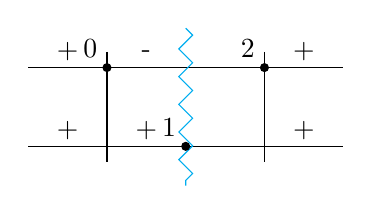
\begin{tikzpicture}
    \draw (-1,0) -- (3,0);
    \draw (-1,-1) -- (3,-1);
    \draw[cyan, decorate, decoration={zigzag}] (1,0.5) -- (1,-1.5);
    \filldraw (0,0) circle (0.05)
      node[above left]{$0$};
    \filldraw (2,0) circle (0.05)
      node[above left]{$2$};
    \filldraw (1,-1) circle (0.05)
      node[above left]{$1$};
    \draw (0,0.2) -- (0,-1.2);
    \draw (2,0.2) -- (2,-1.2);
    \node at (-0.5,0.2){+};
    \node at (0.5,0.2){-};
    \node at (2.5,0.2){+};
    \node at (-0.5,-0.8){+};
    \node at (0.5,-0.8){+};
    \node at (2.5,-0.8){+};
  \end{tikzpicture}
\end{center}
Dato che a noi interessano i strettamente positivi, scriviamo
\begin{equation*}
  \boxed{{]{0},{2}[}}
\end{equation*}

\subsection*{Integrali}

\paragraph{Esercizio 1}
Si risolva
\begin{equation*}
  \int \frac{x}{2x^2+x+1}\,\dif x
\end{equation*}
\divisor

Vediamo un integrale indefinito con una frazione razionale fratta. La prima cosa da fare è 
controllare se il numeratore è la derivata del denominatore
\begin{equation*}
  \Dif (2x^2+x+1) = 4x+1 \neq x
\end{equation*}
No, non è quindi il caso dell'integrale immediato con il logaritmo. Vediamo però che è 
sufficientemente simile, quindi possiamo provare a ricondurlo.
\begin{equation*}
  \int \frac{x}{2x^2+x+1}\,\dif x = \frac{1}{4}\int \frac{4x}{2x^2+x+1}\,\dif x
\end{equation*}
Quasi ma non ancora. Possiamo aggiungere e togliere una stessa quantità però
\begin{equation*}
  \frac{1}{4}\int \frac{4x}{2x^2+x+1}\,\dif x = \frac{1}{4}\int \frac{4x+1-1}{2x^2+x+1}\,\dif x
\end{equation*}
A questo punto possiamo dividere i due integrali
\begin{align*}
  &\frac{1}{4}\int \frac{4x+1-1}{2x^2+x+1}\,\dif x = \frac{1}{4}\int \frac{4x+1}{2x^2+x+1}\,\dif x
  - \frac{1}{4}\int \frac{x}{2x^2+x+1}\,\dif x=\\
  &=\frac{1}{4}\ln\abs{2x^2+x+1} - \frac{1}{4}\int \frac{x}{2x^2+x+1}\,\dif x
\end{align*}
Il secondo integrale ora ovviamente non è nella forma desiderata. Andiammo a calcolare il delta
per vedere quale procedimento seguire
\begin{equation*}
  \Delta = b^2-4ac = 1 - 4\cdot2\cdot1 < 0
\end{equation*}
Ora osserviamo il denominatore
\begin{equation*}
  2x^2+x+1
\end{equation*}
Dobbiamo trovare un numero in modo che si ottenga un quadrato. In questo caso osserviamo che se 
aggiungiamo e togliamo $\frac{1}{8}$
\begin{equation*}
  2x^2+x+\frac{1}{8}-\frac{1}{8}+1 = \left( \sqrt{2}x + \frac{1}{2\sqrt{2}} \right)^2+\frac{7}{8}
\end{equation*}
Possiamo ora continuare il nostro integrale
\begin{equation*}
  \frac{1}{4}\ln\abs{2x^2+x+1} + 
  \frac{1}{4}\int \frac{1}{\left( \sqrt{2}x + \frac{1}{2\sqrt{2}} \right)^2+\frac{7}{8}}\,\dif x
\end{equation*}
A questo punto non resta che riscriverlo in modo che si abbia un qualcosa del tipo 
$\blacksquare^2+1$.
\begin{align*}
  &\frac{1}{4}\ln\abs{2x^2+x+1} - 
  \frac{1}{4}\int \frac{1}{\left(\sqrt{2}x+\frac{1}{2\sqrt{2}}\right)^2+\frac{7}{8}}\,\dif x=\\
  &=\frac{1}{4}\ln\abs{2x^2+x+1} -
  \frac{1}{4}\int \ddfrac{1}{\frac{7}{8}
  \left[1+\ddfrac{\sqrt{2}x+\ddfrac{1}{2\sqrt{2}x}}{\ddfrac{7}{8}}\right]^2}\,\dif x =\\
  &=\frac{1}{4}\ln\abs{2x^2+x+1} -
  \frac{2}{7}\int \ddfrac{1}
  {1+\ddfrac{\left(\frac{4x+1}{2\sqrt{2}}\right)^2}{\left(\sqrt{\frac{7}{8}}\right)^2}}\,\dif x=\\
  &=\frac{1}{4}\ln\abs{2x^2+x+1}-
  \frac{2}{7}\int\ddfrac{1}{1+\left( \frac{4x+1}{\sqrt{7}} \right)^2}\,\dif x =\\
  &=\frac{1}{4}\ln\abs{2x^2+x+1}-
  \frac{1}{2\sqrt{7}}\int\ddfrac{\frac{2}{\sqrt{7}}}{1+\left(\frac{4x+1}{\sqrt{7}}\right)^2}
  \,\dif x =\\
&= \boxed{\frac{1}{4}\ln\abs{2x^2+x+1}-\frac{1}{2\sqrt{7}}\arctan\left(\frac{4x+1}{\sqrt{7}}\right)+k}
\end{align*}
